% last updated in April 2002 by Antje Endemann
% Based on CVPR 07 and LNCS, with modifications by DAF, AZ and elle, 2008 and AA, 2010, and CC, 2011; TT, 2014; AAS, 2016

\documentclass[runningheads]{llncs}
\usepackage{booktabs}
\usepackage{graphicx}
\usepackage{amsmath,amssymb} % define this before the line numbering.
%\usepackage{empheq}
\usepackage{algorithm,algorithmic}

\usepackage{mathrsfs}
\usepackage{epstopdf}
\usepackage{epsfig}

%\usepackage{ruler}
\usepackage{color}
\usepackage[width=122mm,left=12mm,paperwidth=146mm,height=193mm,top=12mm,paperheight=217mm]{geometry}
\usepackage{float,subcaption}
\captionsetup{compatibility=false}

\newtheorem{mydef}{Definition}
\newtheorem{mypro}{Problem}
\newtheorem{mylem}{Lemma}

\begin{document}

% \renewcommand\thelinenumber{\color[rgb]{0.2,0.5,0.8}\normalfont\sffamily\scriptsize\arabic{linenumber}\color[rgb]{0,0,0}}
% \renewcommand\makeLineNumber {\hss\thelinenumber\ \hspace{6mm} \rlap{\hskip\textwidth\ \hspace{6.5mm}\thelinenumber}}
% \linenumbers
\pagestyle{headings}
\mainmatter
\def\rpetitle{Optimal Mass Transport and Its Applications}  % Insert your submission number here

\title{\rpetitle} % Replace with your title

\titlerunning{\rpetitle}

\authorrunning{Junwei Jason Zhang}

\author{Junwei Jason Zhang}
\institute{Ph.D. Preliminary Report \\
Stony Brook University, Stony Brook, NY 11794, USA \\
%\institute{
\vspace{5mm}
-----------------\\
 Committee\\
Xiangmin Jim Jiao, Xianfeng David Gu and Joseph Mitchell}

\maketitle

\begin{abstract}
Optimal Mass Transport Problem (OMT) was first introduced by Monge in 18th century\cite{monge1781memoire},which is presented as a problem minimizing the inter-domain transportation cost while preserving measure quantities. Kantorovich\cite{kantorovich1942transfer} utilized the linear programming approach to prove the existence and uniqueness of the relaxed optimal mass transport(OMT) problem and the space complexity is  $O(n^2)$. In order to increase the time efficiency, we introduced a practical discrete optimal mass transport(OMT) map based on the Brenier's approach\cite{brenier1991polar} and we have proved the  space complexity is $O(n)$.

\keywords{Optimal Mass Transport, Monge-Ampere Equation, Wasserstein Distance, Volume Parameterization}
\end{abstract}

\section{Introduction}

\subsection{Optimal Mass Transportation(OMT)}
\subsubsection{Monge Problem}

In the 18th century, Monge first introduced a problem minimizing the inter-domain transportation cost while preserving measure quantities Fig.[\ref{fig:piles}]. With modern notations, it can be stated as follows:
\begin{mypro}
Given two probability measures $\mu \in \mathbb{P}(X)$ , $\nu \in \mathbb{P}(Y) $, and a cost function $c : X \times Y \rightarrow [0,+\infty]$, solve $$\inf \{M(T) := \int c(x,T(x))d\mu(x): T_{\#}\mu=\nu\}$$
where we recall that the measure denoted by $T_{\#}\mu$, which is defined through $(T_{\#}\mu)(A):=\mu(T^{-1}(A))$ for every A and is called the push-forward of $\mu$ through T.
\end{mypro}

\begin{figure}
\centering
\makebox[\textwidth]{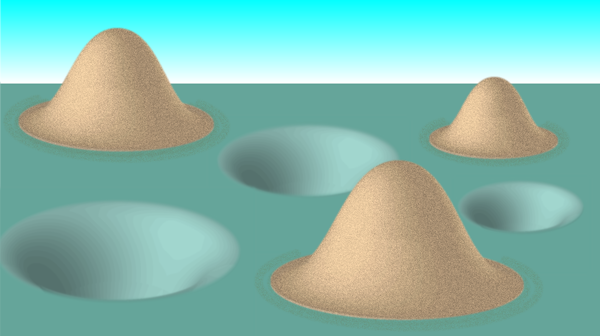
\includegraphics[width=0.5\paperwidth]{figs/piles.png}}
\caption{How do you best move given piles of sand to fill up given holes of the same total volume?}
\label{fig:piles}
\end{figure}


\subsubsection{Kantorovich Problem}

The classical Monge problem solution's existence and uniqueness is not guaranteed. So we consider its relaxed version, which is proposed by Kantorovich \cite{kantorovich1942transfer} :

\begin{mypro}
Given $\mu \in \mathbb{P}(X), \nu \in \mathbb{P}(Y)$ and $c:X\times Y \rightarrow [0,+\infty]$ we consider the problem $$\inf \{K(\gamma):=\int_{X\times Y}c   d\gamma: \gamma \in \Pi(\mu, \nu) \}$$
where $\Pi(\mu, \nu)$ is the set of the so-called transport plans Fig.[\ref{fig:vs}], $$\Pi(\mu,\nu) = \{\gamma \in \mathbb{P}(X\times Y):(\pi_x)_{\#}\gamma = \mu, (\pi_y)_{\#}\gamma = \nu\}$$
where $\pi_x$ and $\pi_y$ are the two projections of $X\times Y$ onto $X$ and $Y$.
\end{mypro}


Alternatively speaking, suppose $X$ and $Y$ are two metric spaces with probability measures $\mu$ , $\nu$, and $X$ , $Y$ have equal total measures:$$\int_X\mu = \int_Y\nu.$$
A map $T:X\rightarrow Y$ is \textit{measure preserving} if for any measurable set $B\subset Y$, it satisfies
\begin{equation}\label{equ2.47}
\mu(T^{-1}(B)) = \nu(B)
\end{equation}
The transportation cost for sending $x\in X$ to $y\in Y$ by $c(x,y)$, then the total \textit{transportation cost} is defined by
\begin{equation}\label{equ2.48}
C(T):=\int_X c(x,T(x))d\mu(x).
\end{equation}

\begin{mypro}
Given two metric spaces with probabilities measure $(X,\mu), (Y,\nu)$ with the transportation cost function $c:X\times Y\rightarrow \mathbb{R}$, the problem is to find the measure preserving map $T:X\rightarrow Y$ satisfying condition (\ref{equ2.47}), which minimizes the transportation cost (\ref{equ2.48}).
\end{mypro}





\subsection{Pioneering Work}

Allen Tannenbaum\cite{haker2004optimal,ur20093d,dominitz2010texture} et al. pioneered the optimal mass transport theory in medical image and computer vision field, whose algorithms are inspired by Kantorovich's approach. Ni\cite{ni2015ricci} et al. applied the optimal mass transport(OMT) theory for internet topology analysis. According to the Computer Graphics applications,Justin Solomon\cite{solomon2015convolutional} et al. have tried their approximate OMT algorithm in shape interpolation and BRDF(Bidirectional Reflectance Distribution Function) acquisition fields. In addition, Bonneel\cite{bonneel2016wasserstein} et al. also tested their Wasserstein Barycentric Coordinates method in shape approximation and color editing applications.

\subsection{Our Approach}

The intrinsic connection between optimal mass transport map and convex geometry was discovered in late 1980's by Brenier\cite{brenier1991polar}, which inspired us from convex geometry's perspective to investigate this problem. Our research approach is written by Gu\cite{gu2013variational} et al., which develops several related finite dimensional variational principles for discrete optimal mass transport, Minkowski type problems for convex polytopes and discrete Monge-Ampere equation. A link between the discrete optimal mass transport, discrete Monge-Ampere equation and the the power diagram in computational geometry is established.


\section{ Theory Background }

In this section, I will introduce the theory background of our research topic, which involves convex geometry, partial differential equation, computational geometry and partial differential geometry. The Fig.[\ref{fig:pipeline}] presents the relationship of different concepts.


\begin{figure}
\centering
\makebox[\textwidth]{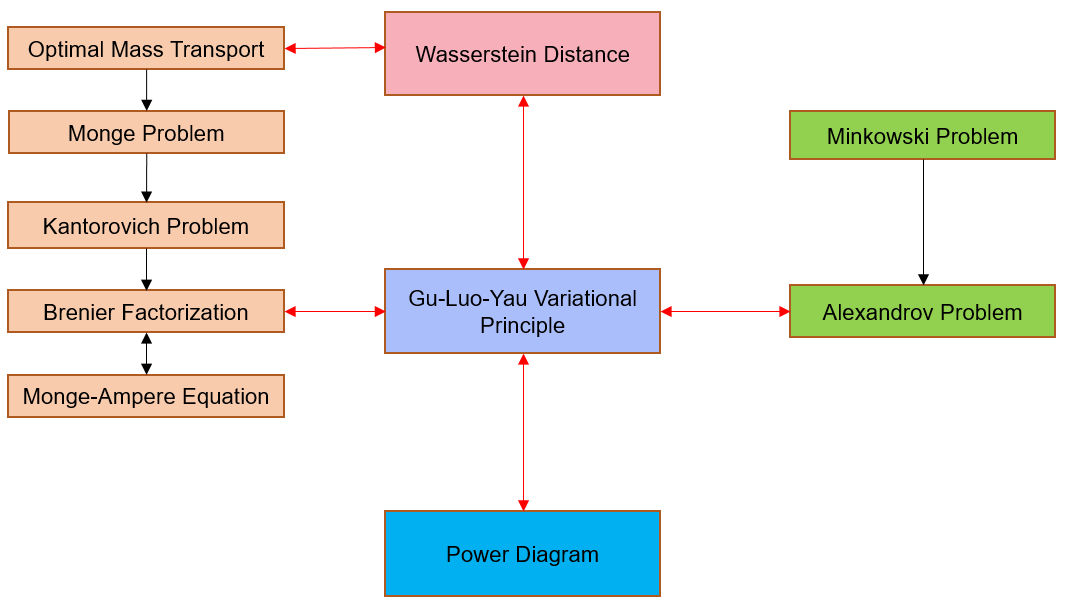
\includegraphics[width=0.7\paperwidth]{figs/pipeline.png}}
\caption{The relationship of theory concepts .}
\label{fig:pipeline}
\end{figure}




\begin{figure}
\centering
\makebox[\textwidth]{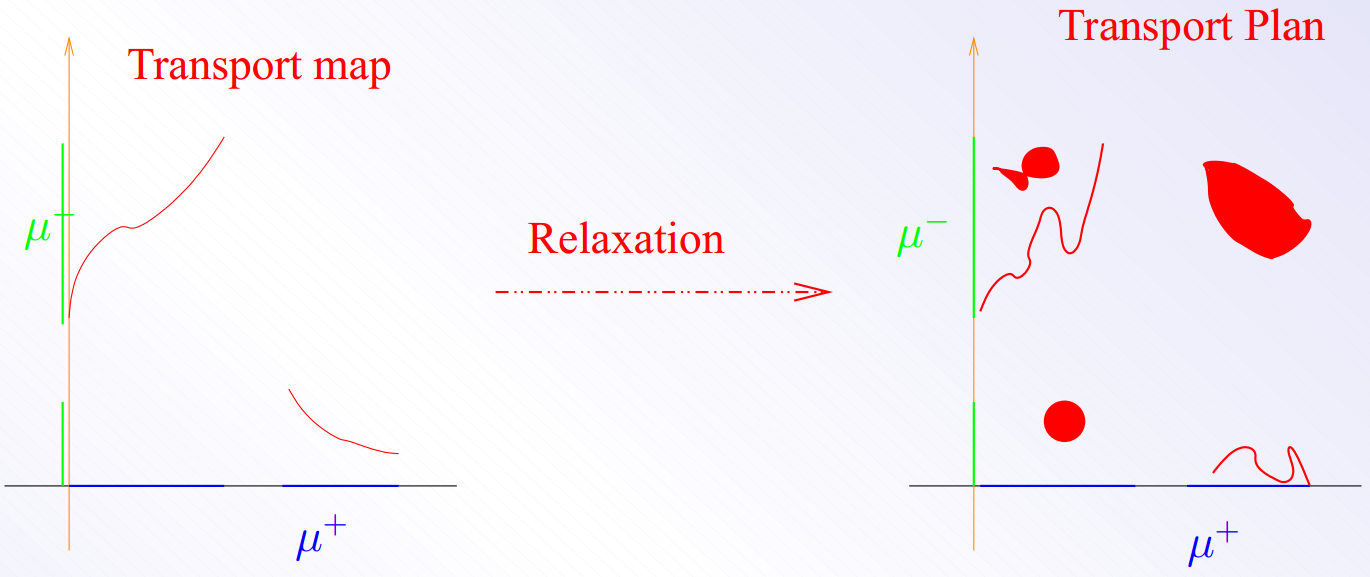
\includegraphics[width=0.7\paperwidth]{figs/map-vs-plan.png}}
\caption{Transport Map vs Transport Plan.}
\label{fig:vs}
\end{figure}




\subsection{Convex Geometry}

\subsubsection{Minkowski Problem}
The classical Minkowski problem for convex polyhedron has influenced the development of convex geometry and differential geometry for decades. One version  Fig.\ref{fig:Mink} of the problem states as following :
\begin{mypro}
Suppose $n_1, n_2, ..., n_k$ are unit vectors which span $\mathbb{R}^n$ and $A_1,..., A_k>0$ so that $\sum^k_{i=1}A_in_i=0$. Find a compact convex polytope $P\subset \mathbb{R}^n$ with exactly k codimension-1 faces $F_1,...,F_k$ so that $n_i$ is the outward normal vector to $F_i$ and the area of $F_i$ is $A_i$.
\end{mypro}

\begin{figure}
\centering
\makebox[\textwidth]{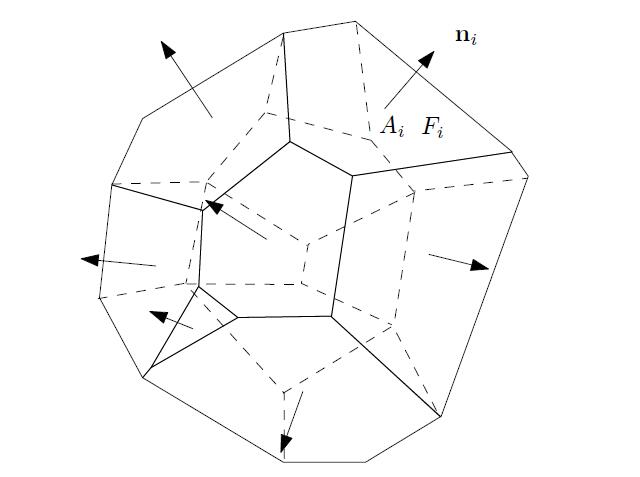
\includegraphics[width=0.5\paperwidth]{figs/MinPro.jpg}}
\caption{Minkowski problem}
\label{fig:Mink}
\end{figure}

Minkowski problem for unbounded convex polytopes was considered and solved by A.D.Alexandrov and A.Pogorelov.

\subsubsection{Alexandrov Problem}

\begin{theorem}
Suppose $\Omega$ is a compact convex polytope with non-empty interior in $\mathbb{R}^n$, $p_1, ... , p_k\subset \mathbb{R}^n$ are distinct k points and $A_1,...,A_k>0$ so that $\sum^k_{i=1}A_i=vol(\Omega)$. Then there exists a vector $h =(h_1,...,h_k)\in \mathbb{R}^k$, unique up to adding the constant$(c,c,...,c)$, so that the piecewise linear convex function$$u(x)=\max_{1\leq i\leq k}\{x\cdot p_i + h_i\}$$ satisfies $vol(\{x\in \Omega | \nabla u(x)=p_i\})=A_i$
\end{theorem}

\begin{figure}
\centering
\makebox[\textwidth]{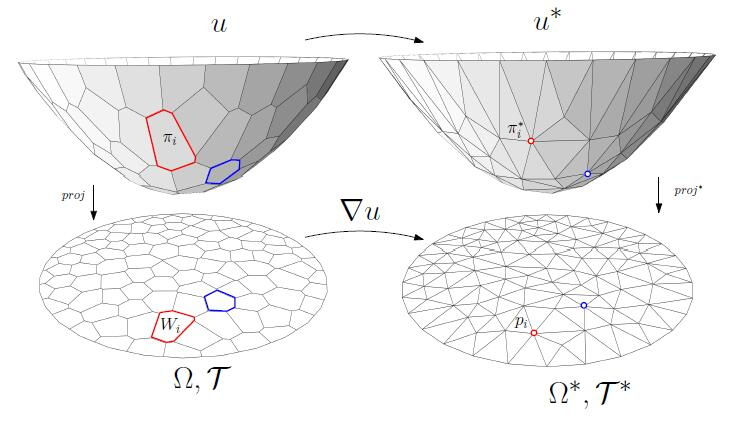
\includegraphics[width=0.5\paperwidth]{figs/AlePro.jpg}}
\caption{A PL convex function induces a cell decomposition of $\Omega$. Each cell maps to a point.}
\label{fig:Alex}
\end{figure}

Alexandrov generalized Minkowski's result to non-compact convex polyhedra. As shown in Fig.\ref{fig:Alex}, given $k$ planes $\pi_i : <x,p_i> + h_i$, one can construct a piecewise linear convex function $$u(x) = \max _i \{<x,p_i>+h_i | i = 1,...,k\}$$ whose graph is an infinite convex polyhedron. The PL convex function produces a convex cell decomposition $\{W_i\}$ of $\mathbb{R}^n$: $$W_i = \{x | <x,p_i>+h_i\geq <x,p_j> +h_j, \forall j\}=\{x|\nabla u(x)=p_i\}$$
Alexandrov shows that the convex polyhedron is determined by the face normal and the projected area $\{A_i\}$.

\subsection{Brenier's Polar Factorization}

\begin{theorem}[Brenier's Polar Factorization\cite{brenier1991polar}]
Let $(X,\mu)$ be a bounded subset of $\mathbb{R}^n$, $h:X \to \mathbb{R}^n$ be an $L^2$ vector-valued mapping satisfying the non-degeneracy condition
\[
\mu(h^{-1}(E)) = 0, \ \textit{for each Lebesgue negligible subset}\ E \subset \mathbb{R}^n
\]
Then there exists a unique measure preserving map $s\in S(X)$ and a unique rearrangement $\nabla \varphi $ of $h$ in the class of $L^2$ gradients of convex functions, such that
\[
h = \nabla \varphi \circ s
\]
$s$ is the unique $L^2$ projection of $h$ onto $S(X)$.
\end{theorem}

\begin{mydef}
(Alexandrov map) The gradient map $\nabla u:x\rightarrow\nabla u(x)$ is the Alexandrov map.
\end{mydef}



\subsection{Monge-Ampere Equation}
Closely related to the optimal mass transport problem is the Monge-Ampere equation(MAE). Let $\Omega$ be a compact domain in $\mathbb{R}^n$, $g:\partial \Omega\rightarrow \mathbb{R}$ and $A:\Omega\times \mathbb{R}\times \mathbb{R}^n\rightarrow\mathbb{R}$ be given. Then the Dirichlet problem for MAE is to find a function $w:\Omega\rightarrow\mathbb{R}$ so that
\begin{equation}\label{eqn:mae}
\left\{
\begin{aligned}
  	& det(Hess(w))(x)=A(x,w(x),\nabla w(x)) \\
	& w|_{\partial\Omega}=g
\end{aligned}
\right.
\end{equation}

where $Hess(w)$ is the Hessian matrix of $w$. We are only interested in solving a discrete MAE in the simplest setting where $A(x,w(x),\nabla w(x))=A(x):\Omega\rightarrow\mathbb{R}$ so that $A(\Omega)$ is a finite set. %$\mathscr{T}$.

We can define the discrete Hessian determinant for piecewise linear function as following:

\begin{mydef}
Suppose(X,$\mathscr{T}$) is a domain in $\mathbb{R}^n$ with a convex cell decomposition $\mathscr{T}$ and $w:X\rightarrow \mathbb{R}$ is a convex function linear on each cell. Then the discrete Hessian determinant of w assigns each vertex $v$ of $\mathscr{T}$ the volume of the convex hull of the gradients of the $w$ at top-dimensional cells adjacent to $v$.
\end{mydef}
Now, we will have the following Dirichlet problem:
\begin{mypro}
\textbf{(Dirichlet problem for discrete MAE)} Suppose $\Omega=conv(v_1, ..., v_m)$ is the convex hull of $v_1,...,v_m$ in $\mathbb{R}^n$. Let $p_1,...,p_k$ be in $int(\Omega)$. Given any $g_1,...,g_m\in\mathbb{R}$ and $A_1,...,A_k>0$, find a convex subdivision $\mathscr{T}$ of $\Omega$ with vertices exactly $\{v_1,...,v_m,p_1,...,p_k\}$ and a PL convex function $w:\Omega\rightarrow \mathbb{R}$ linear on each cell of $\mathscr{T}$ so that
\begin{itemize}
\item[(a)](Discrete Monge-Ampere Equation) the discrete Hessian determinant of $w$ at $p_i$ is $A_i$,
\item[(b)](Dirichlet condition)$w(v_i)=g_i$.
\end{itemize}
\end{mypro}

Then, we have the following theorem for the solution to the equation above:

\begin{theorem}
Suppose $\Omega = conv(v_1,...,v_m)$ is an n-dimensional compact convex polytope in $\mathbb{R}^n$ so that $v_i\notin conv(v_1,...,v_{i-1},v_{i+1},...,v_k)$ for all $i$ and $p_1,...,p_k$ are in the interior of $\Omega$. For any $g_1,...,g_k\in\mathbb{R}$ and $A_1,...,A_k>0$, there exists a convex cell decomposition $\mathscr{T}$ having $v_i$ and $p_j$ as vertices and a piecewise linear convex function $w:(\Omega,\mathscr{T})\rightarrow \mathbb{R}$ so that $w(v_i)=g_i,i=1,...,m$ and the discrete Hessian determinant of $w$ at $p_j$ is $A_j$, $j=1,...,k$. In fact, the solution $w$ is the Legendre dual of $\max\{x\cdot p_j+h_j,x\cdot v_i-g_i|j=1,...,k,i=1,...,m\}$ and $h$ is the unique minimal point of a strictly convex function.
\end{theorem}




\subsection{Optimal Mass Transportation Map by Variational Principle}
According to Monge-Brenier theory\cite{brenier1991polar}, the Alexandrov map is the unique Optimal Mass Transport map that minimizes the following mass transport energy $$\int _\Omega||x-f(x)||^{2}dx$$ among all mass preserving maps $f:\Omega\rightarrow\{p_1,...,p_k\}$, such that $$ Vol(f^{-1}(p_i)) = A_i.$$

The computation of the Alexandrov map is equivalent to computing the \textit{power diagram} in computational geometry.


The computation is based on the following \textit{Generalized Alexandrov Theorem}:

\begin{theorem}
Let $\Omega$ be a compact convex domain in $\mathbb{R}^n$ and $\{p_1,...,p_k\}$ a set of distinct points in $\mathbb{R}^n$ and $\sigma:\Omega \rightarrow \mathbb{R}$ be a positive continuous function. Then for any $A_1,...,A_k>0$ with $\sum^k_{i=1}A_i=\int_\Omega \sigma(x)dx$, there exists $b=(b_1,...,b_k)\in \mathbb{R}^k$, unique up to adding a constant $(c,...,c)$, so that $\int_{W_i(b)\cap\Omega}\sigma(x)dx=A_i$ for all $i$. The vectors b are exactly minimum points of the convex function $$E(h) = \int ^h_a \sum^k_{i=1}\int_{W_i(b)\cap \Omega}\sigma(x)dxdh_i-\sum^k_{i=1}h_iA_i$$
on the open convex set $H={h\in\mathbb{R}^k|vol({W_i(h)\cap \Omega})>0 \forall i}$. In fact, $E(h)$ restricted to $H_0=H\cap\{h|\sum^k_{i=1}h_i=0\}$ is strictly convex. Furthermore, $\nabla u_h$ minimizes the quadratic cost $\int_{\Omega}|x-T(x)|^2\sigma dx$ among all transport maps $T:(\Omega, \sigma dx)\rightarrow(\mathbb{R}^n,\sum^k_{i=1}A_i\delta_{p_i})$
\end{theorem}

In 2D cases, we take $\sigma$ to be the measure density $\rho:\Omega\rightarrow\mathbb{R}$, and $A_i$ to be discrete measures $\mu=\{\mu_1,...,\mu_k\}$. The computation on 2D is based on power diagram and power triangulation. Suppose, two voronoi cells $W_i(\mathbf{h}),W_j(\mathbf{h}) $ are adjacent and share a common edge $e_{ij}$. The edge $e_{ij}$ has a dual Delaunay edge $\bar{e}_{ij}$. The norm with respect to $\rho$ is defined as $$|e|_\rho=\int_{R^3}\rho(x)dx$$ and $|e|$ is just the traditional Euclidean length. By direct computation, we have $$\dfrac{\partial\omega_i}{\partial h_j}=\dfrac{\partial\omega_j}{\partial h_i}=\dfrac{|e_{ij}|_\rho}{|\bar{e}_{ij}|} $$
Therefore, the differential 1-form $\omega=\sum^k_{i=1}\omega_idh_i$ is a closed 1-form, satisfying $d\omega=0$. By Brunn-Minkowski inequality\cite{gardner2002brunn}, the admissible space $H$ is convex and $H \neq \phi$. In addition, $E(h)$ is convex in $h$ and satisfies $$\dfrac{\partial E(h)}{\partial h_i}=\int_{W_i(h)\cap \Omega}\sigma(x)dx.$$

The Hessian matrix of E is defined as follows: $$\dfrac{\partial ^2E}{\partial h_i\partial h_j}=\dfrac{\partial \omega_i}{\partial h_j}=\dfrac{|e_{ij}|_\rho}{|\bar{e}_{ij}|}$$ and the diagonal elements are given by $$\dfrac{\partial \omega_i}{\partial h_i}=-\sum_{i\neq j}\dfrac{\partial \omega_i}{\partial h_j}$$
the negative Hessian matrix is diagonal dominant, so $E$ is concave on admissible space $H$. Therefore the gradient map $\nabla E$ is a diffeomorphism.

The information above gives a guideline of proof\cite{gu2013variational}. Some algorithm details will be discussed in Algorithm section.






\subsection{Area Preserving Mapping}
If we take the measures in the section above as volumes as polyhedra(polyhedrons in 2D case), we will have a conclusion that optimal mass transport map is a special area-preserving mapping, which is defined as follows in the language of differential geometry:

\begin{mydef}
(Area-preserving Mapping). Suppose $\phi:(S_1, \mathbf{g}_1)\rightarrow (S_2, \mathbf{g}_2)$ is a diffeomorphism, the pull back metric induced by $\phi$ on $S_1$ is $\phi^*\mathbf{g}_2$, if $$det(\mathbf{g}_1) = det(\phi^*\mathbf{g}_2) $$ then $\phi$ is an area-preserving mapping.
\end{mydef}


\subsection{Conformal Optimal Mass Transportation}

Given a Riemannian surface $(S,\mathbf{g})$, we can compute a Riemann mapping $\phi:(S,\mathbf{g})\rightarrow(\mathbb{D},dzd\bar{z})$. Assuming the conformal factor function is $\lambda:S\rightarrow \mathbb{R}$, such that $$\mathbf{g}\circ \phi^{-1}(z)=e^{2\lambda(z)}dzd\bar{z}$$
Suppose the total area is $\pi$, such that $$\int_\mathbb{D}e^{2\lambda(z)}dxdy=\pi,$$ we can find the unique optimal mass transportation map(Alexandrov map) $$\tau:(\mathbb{D},e^{2\lambda}dzd\bar{z})\rightarrow(\mathbb{D},d\omega d\bar{\omega}),$$ $\tau$ can be represented as a complex-valued function defined on the unit disk.



\subsection{Wasserstein Distance}

\begin{mydef}
(Shape Distance). Given two Riemannian surfaces, which are topological disks, $(S_1,\mathbf{g}_1)$ and $(S_2,\mathbf{g}_2)$, the Riemann mappings are $\phi_k$, $k=1,2$ respectively. Let $\eta\in  Mob(\mathbb{D})$ be a Mobius transformation, where $Mob(\mathbb{D})$ is the Mobius transformation group of the unit planar disk, then $\eta_k\circ \phi_k$ are still Riemann mappings. Each Riemann mapping $\eta_k\circ \phi_k$ determines a unique optimal mass transportation map $\tau_k(\phi_k,\eta_k)$. Then the distance between two surfaces is given by $$d(S_1,S_2) := \min_{\eta_1,\eta_2\in Mob(\mathbb{D})}\int_\mathbb{D}|\tau_1(\phi_1,\eta_1)-\tau_2(\phi_2,\eta_2)|^2dxdy$$
\end{mydef}

We will show that the Riemann mapping $\phi$ and the optimal mass transportation map $\eta$ encodes all the Riemannian metric information of the original surface by the following lemma:
\begin{mylem}\label{lem:2.1}
Suppose a Riemannian surface $(S,\mathbf{g})$ with a total area $\pi$, which is a topological disk, the Riemann mapping is $\phi:(S,\mathbf{g})\rightarrow (\mathbb{D},dzd\bar{z})$, the conformal factor induced by $\phi$ is $\lambda:S\rightarrow \mathbb{R}$, the optimal mass transportation map is $\eta:(\mathbb{D},e^{2\lambda(z)dzd\bar{z}})\rightarrow (\mathbb{D},dzd\bar{z})$, then the Riemannian metric of the original surface is given by $$\mathbf{g}\circ \phi^{-1}(z)=det(J_\eta)dzd\bar{z}.$$
\end{mylem}
\textit{Proof.} Because $\phi:(S,\mathbf{g})\rightarrow (\mathbb{D},dzd\bar{z})$ is conformal, according to the equation $\phi^*\mathbf{g}_2=e^{2\lambda}\mathbf{g}_1$, we have $$\mathbf{g}\circ \phi^{-1}(z)=e^{2\lambda(z)dzd\bar{z}}.$$
Then, since $\eta:(\mathbb{D},e^{2\lambda(z)dzd\bar{z}})\rightarrow (\mathbb{D},dzd\bar{z})$ is an optimal mass transportation map, it is area-preserving. When we apply the definition of area-preserving mapping, $det(\mathbf{g}_1)=det(\phi^*\mathbf{g}_2)$, we have the following $$e^{2\lambda}=det(J_\eta)$$ Therefore, we have proved the lemma \ref{lem:2.1}.


 Again, we will suppose $(M, \mathbf{g})$ is a Riemannian manifold with a Riemannian metric $\mathbf{g}$. we will focus on the set: $$P_p(M):=\{\mu\in P(M): \int|x|^pd\mu<+\infty\}.$$
For $\mu,\nu\in P_p(M)$, we will define $$W_p(\mu,\nu):=\inf_{T_\#\mu=\nu}(\int_Md(x,T(x))^pd\mu(x))^{\frac{1}{p}}.$$ Then, the quantity $W_p$ defined above is a distance over $P_p(M)$.

\begin{mydef}
(Wasserstein Space). Let $P_p(M)$ denote the space of all probability measures $\mu$ on M with finite $p^{th}$ moment, where $p\geq 1$. Suppose there exists some point $x_0\in M$ that $\int_Md(x,x_0)^pd\mu(x)<+\infty$, where $d$ is the geodesic distance induced by $\mathbf{g}$. We define the Wasserstein space of order $p$ as the space $P_p(M)$, endowed with the distance $W_p$, written as $\mathbb{W}_p$.
\end{mydef}



The following theorem is fundamental for current research.
\begin{theorem}
The Wasserstein distance $W_p$ is a Riemannian metric of the Wasserstein space $\mathbb{W}_p$
\end{theorem}


We now can construct a shape space framework based on optimal mass transport and conformal mapping theories.

We consider all oriented metric surfaces $(M,\mathbf{g})$ with the disk topology, namely $M$ is of genus 0 and with a single boundary $\partial M$. The two markers $\{p,q\}\subset M$, $p$ is an interior point, $q$ is a boundary point. We call $(M,\mathbf{g},p,q)$ as a \textit{marked metric surface}. All marked metric surfaces construct a set $\mathscr{M}$, $\mathscr{M}:=$\{\textit{marked metric surfaces}\}.

We say two marked metric surfaces are equivalent, if there exists a \textit{normalized isometric diffeomorphism} $\phi:(M_1,\mathbf{g}_1,p_1,q_1)\rightarrow (M_2,\mathbf{g}_2,p_2,q_2)$, such that $\phi$ preserves metrics $\phi^*\mathbf{g}_2=\mathbf{g}_1$ and preserves markers $\phi (p_1) = p_2, \phi(q_1)=(q_2)$. The product of the normalized isometry diffeomorphism group and the scaling group is denoted as $G$, $G:=\{normalized \  isometries\}\oplus \{scaling\}$.

Now, we can define the shape space to be a quotient space denoted as $$S:=\mathscr{M}/G.$$

In the following discussion, we always omit the markers \{$p,q$\} in the normalized marked metric surface $(M,\mathbf{g},p,q)\in S$ and assume the total area is $\pi$. According to \textit{Riemann mapping theorem}, there is a unique conformal mapping $\phi:M\rightarrow \mathbb{D}$ with Euclidean metric $dx^2+dy^2$, such that $\phi(p)=(0,0)$ and $\phi(q)=(1,0)$. Then $\mathbf{g}=e^{2\lambda(x,y)}(dx^2+dy^2)$. $\phi$ push forward the area element on $(M,\mathbf{g})$  to the disk $$\mu_{(M,g)}:=e^{2\lambda(x,y)}dx\wedge dy.$$
Then we have an injective mapping $\Gamma:S\rightarrow \mathbb{W}_2(\mathbb{D})$, $\Gamma:(M,\mathbf{g})\mapsto\mu_{(M,\mathbf{g})}.$ The Wasserstein metric on the Wasserstein space $\mathbb{W}_2(\mathbb{D})$ is pulled back to $S$, $$d_S((M_1,\mathbf{g}_1),(M_2,\mathbf{g}_2)):=W_2(\mu(M_1,\mathbf{g}_1),\mu(M_2,\mathbf{g}_2)).$$
We call the metric space $(S,d_S)$ as the \textit{conformal Wasserstein shape space}.

\subsection{Power Diagram}

The Power diagram is a generalization of Voronoi diagram. For a finite set $M\subset E^d$, the \textit{Voronoi diagram} of M associates each $p\in M$ with the convex region $R(p)$ of all points closer to $p$ than to any other point in $M$: $R(p)=\{x\in E^d | d(x,p)<d(x,q), \forall q \in M-\{p\}\}$, where $d$ denotes the Euclidean distance function. If we take the distance function(power function) to be $d(x,p)^2-w(p)$ instead of the standard $L^2$ distance metric, then the Voronoi diagram will become a Power Voronoi diagram. In addition, we write the \textit{power distance} from a point $x\in\mathbb{R}^2$ to $p$ to be as follows: $$POW(x,p_i)=\dfrac{1}{2}||x-p_i||^2-\dfrac{1}{2}h_i$$
When $h_i$ is positive, the intuitive meaning of the power distance is one half of the squred distance from $x$ to the tangent point of $x$ to the circle centered at $p_i$ with radius $\sqrt{h_i}$. The Power Diagram is also a partition of the Euclidean plane into polygonal cells Fig \ref{fig:PowDia}, $$W_i=\{x|Pow(x,p_i)\leq Pow(x,p_j), \forall j\}$$
Comparing with the $W_i$ in Alexandrov problem, it is obvious to see that computing a power diagram is equivalent to compute the Alexandrov map. The computation for discrete situation will be discussed in the next section.

\begin{figure}
\centering
\makebox[\textwidth]{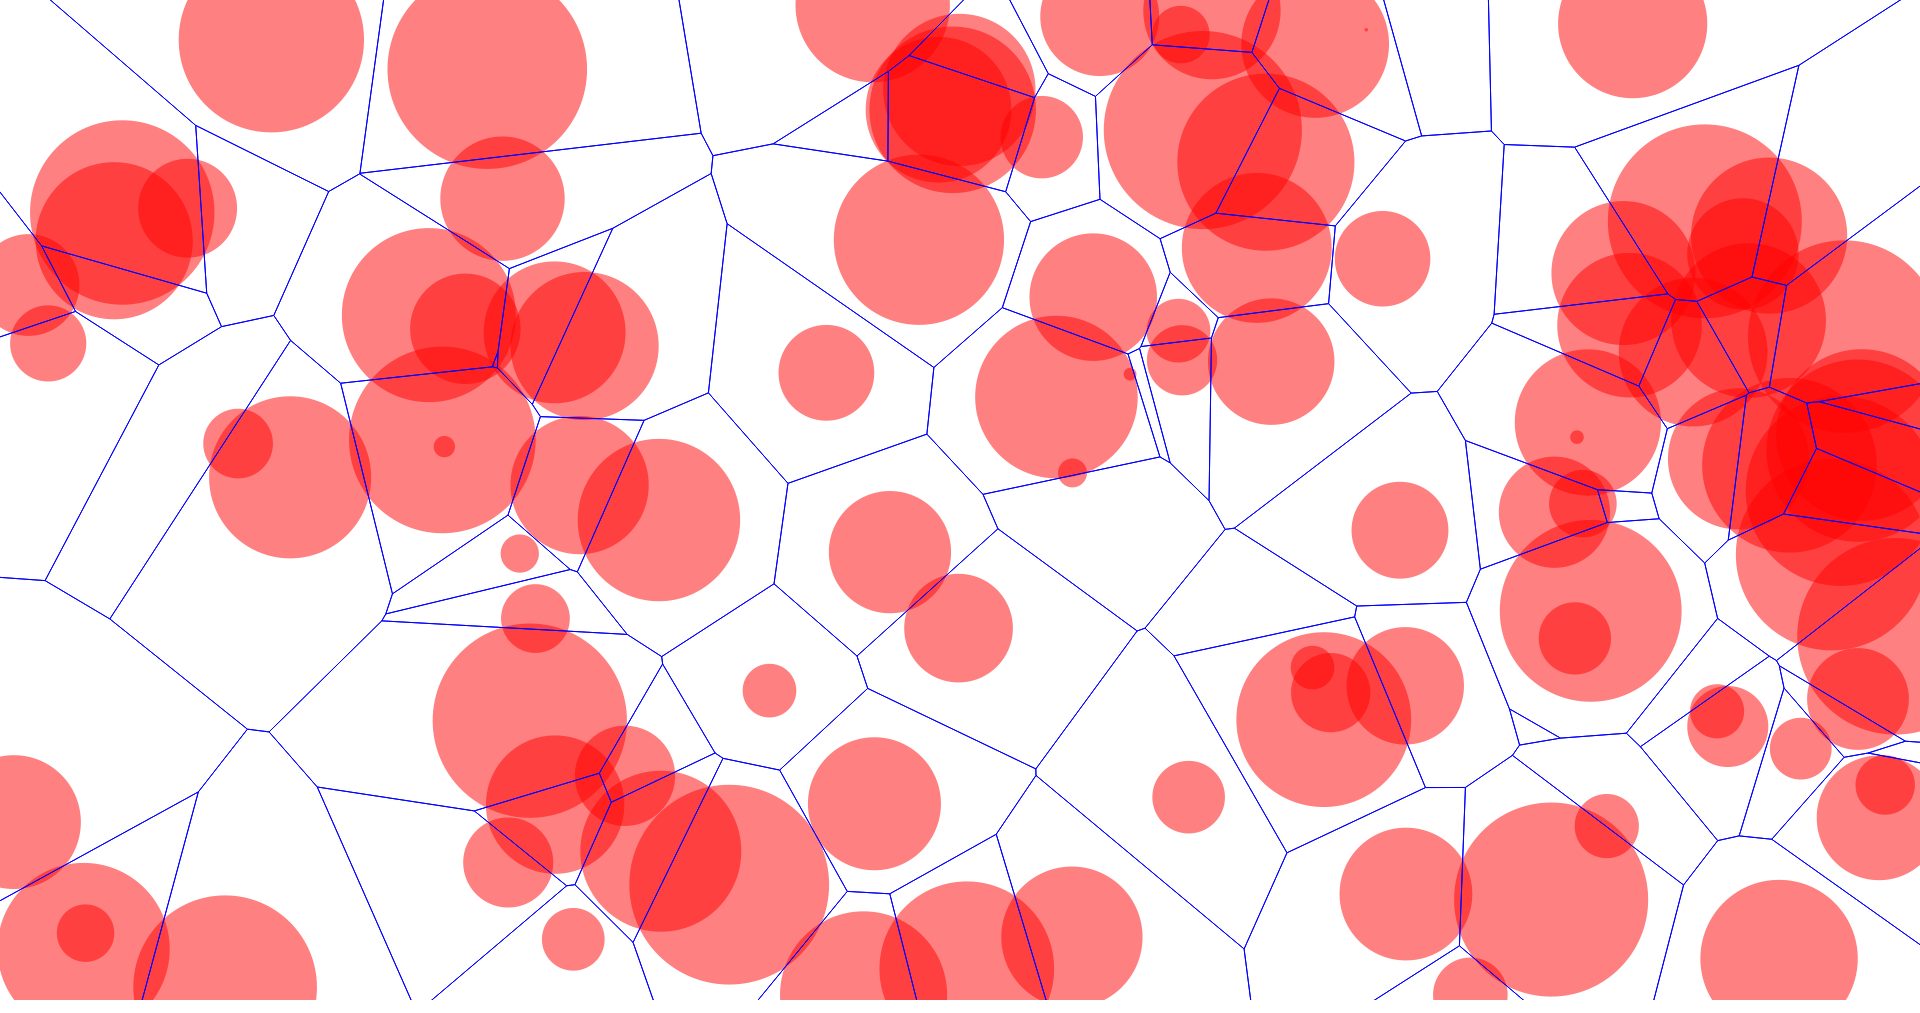
\includegraphics[width=0.6\paperwidth]{figs/full.png}}
\caption{Power diagram.}
\label{fig:PowDia}
\end{figure}

\section{Computational Algorithms In Discrete Settings}

In this section, we present the algorithmic implementation details for conformal mapping and optimal mass transport map(OMT-Map) generation. Based on the OMT-Map algorithm, we introduce surface area-preserving parameterization algorithm on simply connected surfaces, and the computation for conformal Wasserstein distance between surfaces.

In discrete settings, surfaces are represented as discrete polyhedral patches. Suppose $S$ is a topological surface, $V$ is a set of points on $S$, $(S,V)$ is called a \textit{marked surface}. $T$ is a triangulation of $S$, whose vertices are in $V$, then $(S,T)$ is called a \textit{triangular mesh}. In the following discussion, we use $V$, $E$ and $F$ to represent the set of \textit{vertices, edges, and faces}. A piecewise linear Riemannian metric (PL metric) on $(S,V)$ is a flat cone metric, whose cone points are in $V$, represented by edge lengths.

\subsection{Discrete Conformal Mapping}


\begin{mydef}
(Discrete Riemannian Metric). A discrete metric on a triangular mesh $(S,T)$ is a function defined on the edges $d:E\rightarrow \mathbb{R}^+$, which satisfies the triangle inequality, on a face $[v_i,v_j,v_k]$, $$d_{ij}+d_{jk}>d_{ki};d_{ki}+d_{ij}>d_{jk};d_{ik}+d_{kj}>d_{ji}.$$
\end{mydef}

\begin{mydef}
(Discrete Gauss Curvature). The discrete Gauss curvature function on a mesh is defined on vertices, $K: V\rightarrow \mathbb{R}$, such that
\[
	K(v)=\begin{cases}
			2\pi-\sum_i\theta_i,\ v\notin\partial S\\
			\pi-\sum_i\theta_i, \ v\in\partial S
		\end{cases}			
\]
where $\theta_i$'s are corner angles adjacent to the vertex $v$, and $\partial S$ represents the boundary of the mesh.
\end{mydef}

Gauss-Bonnet theorem still holds on discrete surface as following: $$\sum_i K(v_i)=2\pi\chi(S)$$
where $\chi(S)$ is the Euler characteristic of $S$.


\begin{mydef}
(Delaunay Triangulation). A closed discrete surface $(S,T)$ with a discrete metric $d$, we say a triangulation $T$ is Delaunay, if for any edge $[v_i,v_j]$ adjacent to two faces $[v_i,v_j,v_k]$ and $[v_j,v_i,v_l]$, $$\theta_k^{ij}+\theta_l^{ji}\leq \pi,$$ where $\theta_k^{ij}$ is the corner angle at $v_k$ in $[v_i,v_j,v_k]$, and $\theta_l^{ji}$ is the angle at $v_l$ in $[v_j,v_i,v_l]$.
\end{mydef}



\subsection{Discrete Yamabe Flow}
The first algorithm presented here is the \textit{discrete surface Yamabe flow} algorithm. We define the discrete conformal factor function as $u: V\rightarrow \mathbb{R}$, and conformal structure coefficient on edges $\eta:E\rightarrow \mathbb{R}^+$.
\begin{mydef}
(Discrete Yamabe Flow with Surgery). Given a surface $(S,V)$ with a discrete metric $d$, given a target curvature function $\bar{K}:V\rightarrow \mathbb{R},\ \bar{K}(v_i)\in(-\infty,2\pi)$, and the total target curvature satisfies Gauss-Bonnet formula, the discrete Yamabe flow is defined as $$\dfrac{du(v_i)}{dt}=\bar{K}(v_i)-K(v_i),$$
under the constraint $\sum_{v_i\in V}u(v_i) = 0$. During the flow, the triangulation on $(S,V)$ is updated to be Delaunay with respect to $d(t)$, for all time t.
\end{mydef}

The following theorem guarantees the existence of the solution to the Yamabe flow.

\begin{theorem}
Suppose $(S,V)$ is a closed connected surface and $d$ is any discrete metric on $(S,V)$. Then for any $\bar{K}:V\rightarrow (-\infty,2\pi)$ satisfying Gauss-Bonnet formula, there exists a discrete metric $\bar{d}$, unique up to a scaling on $(S,V)$, so that $\bar{d}$ is discrete conformal to $d$ and the discrete curvature of $\bar{d}$ is $\bar{K}$. Furthermore, the $\bar{d}$ can be obtained by discrete Yamabe flow with surgery.
\end{theorem}

It is known that that Yamabe flow is the negative gradient flow of the following Yamabe energy: $$f(u_1,u_2,...,u_n)=\int^{(u_1,u_2,...,u_n)}\sum_{v_i\in V}(\bar{K}(v_i)-K(v_i))du_i$$
The gradient of the energy is $\nabla f(u_1,u_2,...,u_n)=(\bar{K}(1)-K(1),...,\bar{K}(n)-K(n))^T$. The Hessian matrix is formulated as $H = (h_{ij})$, satisfying
\[
	h_{ij} = \begin{cases}
			-w_{ij} & v_i\sim v_j\  i\neq j \\
			0  &v_i\nsim v_j \ i\neq j \\
			\sum_k w_{ik}  &i=j
		\end{cases}
\]
where $w_{ij}$ is the cotangent edge weight defined as
\[
w_{ij} := \begin{cases}
		cot\theta^{ij}_k+cot\theta^{ji}_l &[v_i,v_j]\notin \partial S \\
		cot\theta^{ij}_k &[v_i,v_j]\in \partial S
	\end{cases}
\]

\begin{algorithm}
\caption{Discrete Surface Yamabe Flow}
\begin{algorithmic}[1]
	\REQUIRE The inputs include:
	\begin{enumerate}
	\item[1.] A triangular mesh $\Sigma$, embedded in $\mathbb{E}^3$
	\item[2.] A target curvature $\bar{K}$, satisfying Gauss-Bonnet formula.
	\end{enumerate}
	\ENSURE: A discrete metric conformal to the original one, satisfying the target curvature $\bar{K}$.
  	\STATE Initialize the discrete conformal factor $u$ as 0 and conformal structure coefficient $\eta$, such that $\eta(e)$ equals to the initial edge length of $e$.
  	\WHILE{$\max_i|\bar{K}_i-K_i|>\epsilon$}
  	\STATE compute the edge length from $\gamma$ and $\eta$
  	\STATE Update the triangulation to be Delaunay using diagonal edge swap for each pair of adjacent faces
  	\STATE Compute the corner angle $\theta^{jk}_i$ from the edge length using cosine law
  	\STATE Compute the vertex curvature $K$
  	\STATE Compute the Hessian matrix $H$
  	\STATE Solve linear system $H\delta u=\bar{K}-K$
  	\STATE Update conformal factor $u\leftarrow u-\delta u$
  	\ENDWHILE
  	\STATE Output the result circle packing metric
\end{algorithmic}
\label{Algo:yamabe}
\end{algorithm}

Newton's method is used when optimizing the Yamabe energy to compute the conformal metric with prescribed curvature.




\subsection{Discrete Optimal Mass Transport}

Now, we will present the Discrete version of the Optimal Mass Transport theory.


\subsubsection{Kantorovich's Approach.}

The main idea of Kantorovich's approach is to simplify the OMT problem to a linear programming problem with $n^2$ unknowns.

Suppose space $X$ and $Y$ are discretized to sample points, $X=\{x_1,x_2,...,x_n\}$, $Y=\{y_1,y_2,...,y_n\}$, the measures are dirac measures $$\mu=\sum^n_{i=1}\mu_i\delta(x-x_i),\nu=\sum^n_{j=1}\nu_i\delta(y-y_i),$$
the transport plan $f$ is represented as a matrix $(f_{ij})$, such that $$\sum^n_{j=1}f_{ij}=1,\sum^n_{i=1}f_{ij}=1,f_{ij}\geq 0.$$
All such matrices form a convex polytope, and the total transportation cost becomes a linear function $$C(f)=\sum_{i,j}c(x_i,y_i)f_{ij}.$$

Obviously, this linear programming problem has $n^2$ unknowns $f_{ij}$.

\subsubsection{Brenier's Approach}

Suppose $\mu$ has a compact support on $X$, define the domain $$\Omega = sup\ \mu={x\in X|\mu(x)>0},$$ assume $\Omega$ is a convex domain in $X$. The space $Y$ is discretized to $Y=\{y_1,y_2,...,y_k\}$ with Dirac measure $\nu =\sum^k_{j=1}\nu_j\delta(y-y_j).$

We will define a height vector $\mathbf{h}=(h_1,h_2,...,h_k)$ and for each $y_i\in Y$, we define a hyperplane defined on X, $$\pi_i(\mathbf{h}):<x,y_i>+h_i=0.$$

Define a convex function as following: $$u_\mathbf{h}(x)=\max^k_{i=1}\{<x,y_i>+h_i\}$$

We denote its graph by $G(\mathbf{h})$, which is an infinite convex polyhedron with supporting planes $\pi_i(\mathbf{h})$. The projection of $G(\mathbf{h})$ induces a polygonal partition of $\Omega$, $$\Omega = \cup^k_{i=1}W_i(\mathbf{h})$$ where each cell $W_i(\mathbf{h})$ is defined as the projection of a facet of the convex polyhedron $G(\mathbf{h})$ onto $\Omega$, $W_i(\mathbf{h})=\{x\in X|u_{\mathbf{h}}(x) = <x,y_i>+h_i\}\cap \Omega$. And the area of $W_i$ is given by $w_i(\mathbf{h})=\int_{W_i}(\mathbf{h})\mu(x)dx.$ Since the convex function $u_{\mathbf{h}}$ on each cell $W_i(\mathbf{h})$ is a linear function $\pi_i(\mathbf{h})$, the gradient map $$ \nabla\ u_\mathbf{h}:W_i(\mathbf{h})\rightarrow y_i, \ i=1,2,...,k.$$ maps each $W_i(\mathbf{h})$ to a single point $y_i$.

Using the formula and definition above, we will present a theorem that plays a fundamental role for discrete optimal mass transport theory:
\begin{theorem}
For any given measure $\nu$, such that $$\sum^n_{j=1}\nu_j=\int_\Omega \mu, \nu_j>0,$$ there must exist a height vector $\mathbf{h}$ unique up to adding a constant vector $(c,c,...,c)$, the convex function $u_\mathbf{h}(x)$ induces the cell decomposition of $\Omega = \cup^k_{i=1}W_i(\mathbf{h})$, such that the folloing area-preserving constraints are satisfied for all cells, $$\int_{W_i(\mathbf{h})}=\nu_i,\ i=1,2,...,n. $$
Furthermore, the gradient map $grad\ u_{\mathbf{h}}$ optimizes the transportation cost $$C(T):=\sum_\Omega|x-T(x)|^2\mu(x)dx.$$
\end{theorem}

Recently, Gu\cite{gu2013variational} gives a novel proof for the existence and uniqueness based on the variational principle for the following discrete version of Brenier's approach.
\begin{theorem}
Let $\Omega$ be a compact convex domain in $\mathbb{R}^n$, $\{p_1,...,p_k\}$ be a set of distinct points in $\mathbb{R}^n$ and $\sigma:\Omega\rightarrow \mathbb{R}$ be a positive continuous function. Then for any $A_1,...,A_k>0$ with $\sum^k_{i=1}A_i=\int_{\Omega}\sigma(x)dx,$ there exists $b=(b_1,...,b_k)\in \mathbb{R}^k$, unique up to adding a constant $(c,c,...,c)$, so that $\int_{W_i(b)\cap \Omega}sigma(x)dx=A_i$ for all $i$. The vectors $b$ are exactly minimum points of the convex function $$E(h)=\int^h_a\sum^k_{i=1}\int_{W_i(h)\cap\Omega}\sigma(x)dxdh_i-\sum^k_{i=1}h_iA_i$$ on the open convex set $H=\{h\in\mathbb{R}^k|vol(W_(h)\cap \Omega)>0\ for\ all\ i\}$. Furthermore, $\nabla u_b$ minimizes the quadratic cost $\int_\Omega|x-T(x)|^2\sigma(x)dx$ among all transport maps $T:(\Omega,\sigma dx)\rightarrow(\mathbb{R}^n,\sum^k_{i=1}A_i\delta_{p_i})$
\end{theorem}
\begin{theorem}
(Discrete OMT) If $\Omega$ is convex, then the admissible space $H_0$ is convex, so is the energy $E(\mathbf{h})$, where $$E(\mathbf{h})=\int_\Omega u_\mathbf{h}(x)\mu(x)dx-\sum^k_{i=1}\nu_i h_i.$$ In addition, the unique global minimum $\mathbf{h}_0$ is an interior point of $H_0$. And the gradient map $ \nabla\ u_\mathbf{h}$ induced by the minimum $\mathbf{h}_0$ is the unique optimal mass transport map, which minimizes the total transportation cost $C(T)$.
\end{theorem}



\subsubsection{Optimal Mass Transport Map Algorithm}
Assume $\Omega$ is a convex planar domain with measure density $\mu$, $P=\{p_1,...,p_k\}$ is a point set with measure $\nu=\{\nu_1,...,\nu_k\}$, such that $\int_\Omega \mu(x)dx=\sum^k_{i=1}\nu_i$. In practice, the energy can be optimized using Newton's method, with the help of the computation of the energy gradient$\nabla E(\mathbf{h})=(w_1(\mathbf{h})-\nu_1),...,w_k(\mathbf{h})-\nu_k)^T$. The Hessian of $E(\mathbf{h})$ is given as following:
\[
\dfrac{\partial ^2E(\mathbf{h})}{\partial h_i\partial h_j}=\begin{cases}
					\frac{\int_{e_{ij}}\mu(x)dx}{|y_j-y_i|}\ &W_i(\mathbf{h})\cap W_j(\mathbf{h})\cap \Omega\neq\emptyset \\
					0 &otherwise
\end{cases}
\]






\begin{algorithm}
\caption{Optimal Mass Transport Map}
\begin{algorithmic}[1]
	\REQUIRE \textbf{Input:}
	\begin{enumerate}
	\item[1.] A convex planar domain with measure $(\Omega,\mu)$;
	\item[2.] A planar point set with measure $(P,\nu),\nu_i>0,\int_\Omega u(x)dx=\sum^k_{i=1}\nu_i$
	\end{enumerate}
	\textbf{Output:} The unique discrete OMT-Map $f:(\Omega,\mu)\rightarrow(P,\nu)$
	
  	\STATE Scale and translate P, such that $P\subset \Omega$
  	\STATE $\mathbf{h}\leftarrow(0,0,...,0)$
  	\STATE Compute the power diagram $D(\mathbf{h})$
  	\STATE Compute the dual power Delaunay triangulation $T(\mathbf{h})$
  	\STATE Compute the cell areas $\mathbf{w}(\mathbf{h})=(w_1(\mathbf{h}),...,w_k(\mathbf{h}))$
  	\WHILE{$||\nabla E||<\epsilon$}
  	\STATE Compute $\nabla E$
  	\STATE Compute the Hessian matrix
  	\STATE $\lambda\leftarrow 1$
  	\STATE $\mathbf{h}\leftarrow \mathbf{h}-\lambda H^{-1}\nabla E(\mathbf{h})$
  	\STATE Compute $D(\mathbf{h})$, $T(\mathbf{h})$, and $\mathbf{w}(\mathbf{h})$
  		\WHILE{$\exists w_i(\mathbf{h})==0$}
  		\STATE $\mathbf{h}\leftarrow \mathbf{h}+\lambda H^{-1}\nabla E(\mathbf{h})$
  		\STATE $\lambda\leftarrow\frac{1}{2}\lambda$
  		\STATE $\mathbf{h}\leftarrow \mathbf{h}-\lambda H^{-1}\nabla E(\mathbf{h})$
  		\STATE Compute $D(\mathbf{h})$, $T(\mathbf{h})$, and $\mathbf{w}(\mathbf{h})$
  		\ENDWHILE
  	\ENDWHILE
  	\STATE Output the result mapping $f:\Omega\rightarrow P, W_i(\mathbf{h})\rightarrow p_i,\ i=1,2,...,k.$
\end{algorithmic}
\label{Algo:OMT}
\end{algorithm}




\subsection{Area Preserving Map For Topological Disks}

The area-preserving mapping is a generalization of the OMT mapping algorithm. Suppose $S$ is a topological disk, with a Riemannian metric $\mathbf{g}$. By scaling, the total area of $(S,\mathbf{g})$ can be equal to $\pi$. According to Riemann Mapping theorem, there is a conformal mapping $\phi :(S,\mathbf{g})\rightarrow(\mathbb{D},dzd\bar{z})$, such that $\mathbf{g}= e^{2\lambda(z)}dzd\bar{z}$. Then we can find the OMT map $\tau:(\mathbb{D},dzd\bar{z})\rightarrow (\mathbb{D},e^{2\lambda}dzd\bar{z})$, and the composition $\tau^{-1}\circ \phi:(S,\mathbf{g})\rightarrow(\mathbb{D},dzd\bar{z})$ gives the area-preserving mapping.

\begin{algorithm}\label{Algo:DiskOMT}
\caption{Topological Disk Area-preserving Parameterization}
\begin{algorithmic}[1]
	\REQUIRE \textbf{Inputs:} a triangular mesh $M$, which is a topological disk; three vertices $\{v_0,v_1,v_2\}\subset \partial M$ \\
	\textbf{Output:} The area-preserving parameterization $f:M\rightarrow \mathbb{D}$, which maps $\{v_0,v_1,v_2\}$ to $\{1,i,-1\}$ respectively.
	\STATE Scale $M$ such that the total area is $\pi$
	\STATE Compute the conformal parameterization $\phi:M\rightarrow\mathbb{D}$, such that the images of $\{v_0,v_1,v_2\}$ are $\{1,i,-1\}$
	\STATE For each vertex $v_i\in M$, define $p_i=\phi(v_i)$, $\nu_i$ to be $\frac{1}{3}$ of the total area of the faces adjacent to $v_i$. Set $P=\{p_i\},\nu=\{\nu_i\}$
	\STATE Compute the \textit{Discrete Optimal Mass Transport Map}
	\STATE Construct the mapping $\tau^{-1}\circ\phi:M\rightarrow\mathbb{D}$, which maps each vertex $v_i\in M$ to the centroid of $W_i(\mathbf{h})\subset \mathbb{D}$	
	
\end{algorithmic}
\end{algorithm}


\subsubsection{Conformal Wasserstein Distance}
The OMT-Map algorithm can also be generalized to compute the Wasserstein distance between surfaces. Given two topological disk surfaces $(M_1,g_1,p_1,q_1)\in S, (M_2,g_2,p_2,q_2)\in S$ with total area $\pi$, where $S$ is the normalized marked metric space, $p_1, p_2$ are correspondent interior markers, and $q_1, q_2$ are markers on the boundary. We first compute the conformal maps $\phi_1:M_1\rightarrow \mathbb{D}_1$, and $\phi_2:M_2\rightarrow \mathbb{D}_2$, where $\mathbb{D}_1$ and $\mathbb{D}_2$ are unit planar disks with Euclidean metric $dx^2+dy^2$, such that $\phi(p_1)=\phi(p_2)=(0,0)$ and $\phi(q_1)=\phi(q_2)=(1,0).$ Then we construct a convex planar domain $(\Omega, \mu)$ from $\mathbb{D}_1$. Then we discretize $\mathbb{D}_2$ into a planar point set with measure $(P,\nu)$, where $\nu_i=\dfrac{1}{3}\sum_{[v_i,v_j,v_k]\in M}area([v_i,v_j,v_k)$. Using $(\Omega,\mu)$ and $(P,\nu)$ as input for Algorithm \ref{Algo:OMT}, we can compute the OMT map $f:\Omega\rightarrow P, W_i(\mathbf{h})\rightarrow p_i$. Therefore, the Wasserstein distance between $M_1$ and $M_2$ can be computed by $$d_W(\mu,\nu)=\sum^n_{i=1}\int_{W_i}(x-p_i)^2\mu(x)dx$$

\begin{algorithm}\label{Algo:WasDis}
\caption{Computing Wasserstein Distance for Two Surfaces}
\begin{algorithmic}[1]
\REQUIRE \textbf{Inputs:} Two topological disk surfaces:$(M_1,g_1,p_1,q_1), (M_2,g_2,p_2,q_2)$, parameters defined as above. \\
\textbf{Outputs:} The Wasserstein distance between $M_1$ and $M_2$
\STATE Scale and normalize $M_1$ and $M_2$ such that the total area of each is $\pi$.
\STATE Compute the conformal maps $\phi_1:M_1\rightarrow \mathbb{D}_1$, and $\phi_2:M_2\rightarrow \mathbb{D}_2$ defined above.
\STATE Construct the convex planar domain $(\Omega,\mu)$ from $\mathbb{D}_1$
\STATE Discretize $\mathbb{D}_2$ into a planar point set with measure $(P,\nu)$
\STATE With $(\Omega, \mu)$ and $(P,\nu)$ as inputs, compute the Optimal Mass Transport map $f$ with Algorithm 2
\STATE Output the Wasserstein distance $d_W(\mu,\nu)$.
\end{algorithmic}
\end{algorithm}

\clearpage



\begin{algorithm}[H]
\caption{Polar Factorization of Mapping}
\begin{algorithmic}
\REQUIRE Convex domains $\Omega_0$ and $\Omega_1$ in $\mathbb{R}^d$. A diffeomorphic mapping $\phi:(\Omega_0,\mu_0)\rightarrow (\Omega_1, \mu_1)$, satisfying $\mu_1=\phi_\#\mu_0$.
\ENSURE The polar factorization $\phi = \nabla u\circ s$, where $s$ is measure-preserving and $u$ is convex.
\STATE Compute the unique optimal mass transport map $\nabla v:(\Omega_1, \mu_1)\rightarrow (\Omega_0,\mu_0)$ using Alg.\ref{Algo:OMT}. The convex function $u$ is the Legendre dual of $v$, $u=v^*$
\STATE Compute the composition $s=\nabla v\circ\phi$
\end{algorithmic}
\label{Algo:PolarFac}
\end{algorithm}




\section{Applications}


In this section, I present three applications based on or derived from the \textit{Optimal Mass Transport} theory.


\subsection{Wasserstein Distance for Shape Analysis}

In our paper,a novel shape classification method for brain's hippocampus is proposed. Table[\ref{fig:textures}] and Fig.[\ref{fig:ROC1}] [\ref{fig:ROC2}] demonstrate our method has better classification performance than other methods.

\setlength{\tabcolsep}{2mm}
\begin{figure*}[!t]
\begin{center}
\begin{tabular}{cccc}
\epsfig{file=./figs/normal_left_checkerboard.eps,width=0.225\textwidth}&
\epsfig{file=./figs/normal_right_checkerboard.eps,width=0.225\textwidth}&
\epsfig{file=./figs/epilepsy_left_checkerboard.eps,width=0.225\textwidth}&
\epsfig{file=./figs/epilepsy_right_checkerboard.eps,width=0.225\textwidth}\\
(a) & (b) & (c) & (d)\\
\epsfig{file=./figs/normal_left_circle.eps,width=0.225\textwidth}&
\epsfig{file=./figs/normal_right_circle.eps,width=0.225\textwidth}&
\epsfig{file=./figs/epilepsy_left_circle.eps,width=0.225\textwidth}&
\epsfig{file=./figs/epilepsy_right_circle.eps,width=0.225\textwidth}\\
(e) & (f) & (g) & (h)\\
\end{tabular}
\end{center}
\caption{Conformal texture-mapping results. (a)-(d)
conformal checkerboard-texture mapping results of left and right hippocampus
surfaces in normal control and epilepsy data groups, respectively; (e)-(h)
conformal circle-texture mapping results of left and right hippocampus
surfaces in normal control and epilepsy data groups, respectively.}
\label{fig:textures}
\end{figure*}




\begin{figure*}[!t]
\begin{minipage}[!t]{0.44\textwidth}
\includegraphics[width=\textwidth]{figs/ROC1.eps}
\caption{Comparison of average ROC curves for three methods.}\vspace{3em}
\label{fig:ROC1}
\end{minipage}%
\hspace{.3in}
\begin{minipage}[!t]{0.47\textwidth}
\includegraphics[width=\textwidth]{figs/ROC2.eps}
\caption{Comparison of average ROC curves between our method and the combination of the other two methods.}
\label{fig:ROC2}
\end{minipage}
\end{figure*}



\begin{table}
\centering
\caption{Average AUC value.}
\label{tbl:ROC}
\begin{tabular}[\textwidth]{@{\extracolsep{\fill}}lc}
\hline
Methods & Average AUC value\\
\hline
Area Distortion& 0.6948 \\
Curvature Difference & 0.7342\\
Curvature Difference + Area Distortion & 0.7542\\
Wasserstein Distance & 0.8834\\
\hline
\end{tabular}
\end{table}





\subsection{Optimal Mass Transport For Visualization}
Our work\cite{su2016area} allows users to fully control the texture area of region of interests, which will be helpful in medical image field. By adjusting the target measure, the user can zoom or shrink specific regions on the surface as shown in Fig. [\ref{fig:roi_face}] and [\ref{fig:roi_skull}].
The top row demonstrates that the user can control the areas of the holes, the bottom row shows the user can enlarge/shrink the nose region with different scaling factors in \ref{fig:roi_face}. The similar observation is also obtained from skull model shown in \ref{fig:roi_skull}.


{ \setlength{\tabcolsep}{0pt}
\begin{figure}[!htbp]
\centering
\begin{tabular}{cccc}
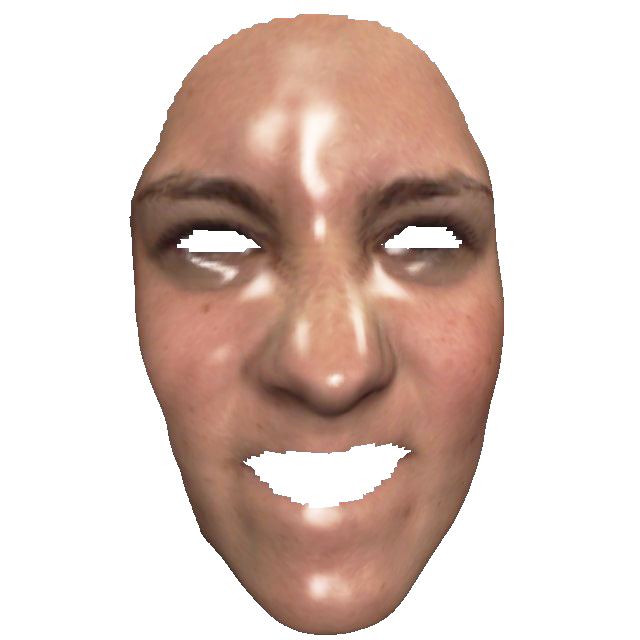
\includegraphics[height=0.25\textwidth]{./figs/roi_face/face_a.jpg}&
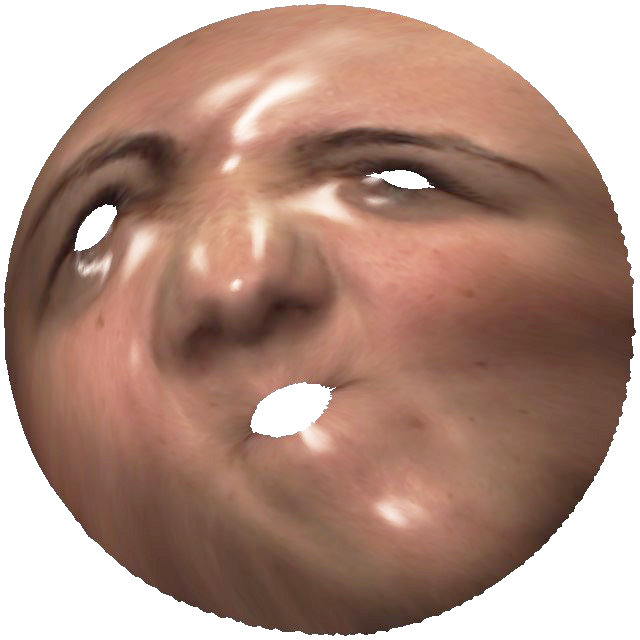
\includegraphics[height=0.25\textwidth]{./figs/roi_face/face_b.jpg}&
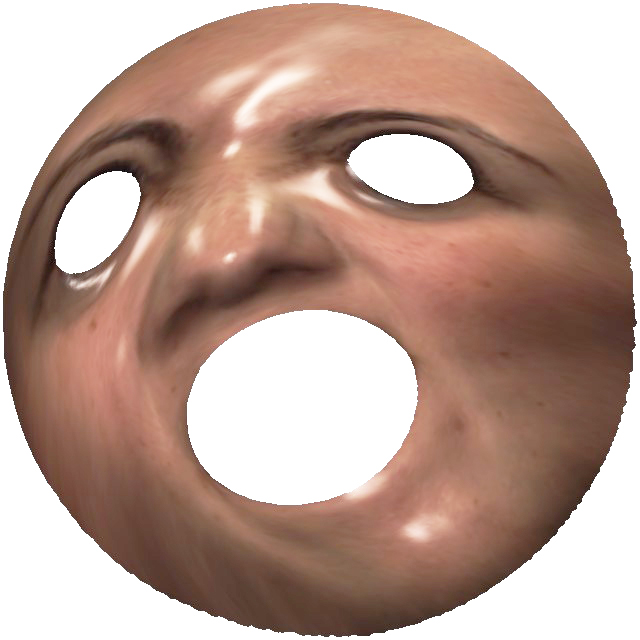
\includegraphics[height=0.25\textwidth]{./figs/roi_face/face_c.jpg}&
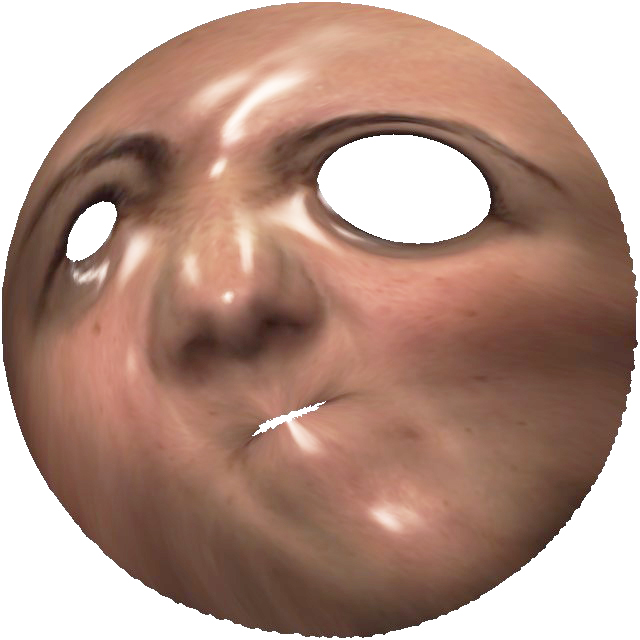
\includegraphics[height=0.25\textwidth]{./figs/roi_face/face_d.jpg}\\
(a)3D face model&(b) holes:0.25X &(c) holes:4X &(d) holes:1X,8X,0.01X \\
\end{tabular}
\begin{tabular}{cccc}
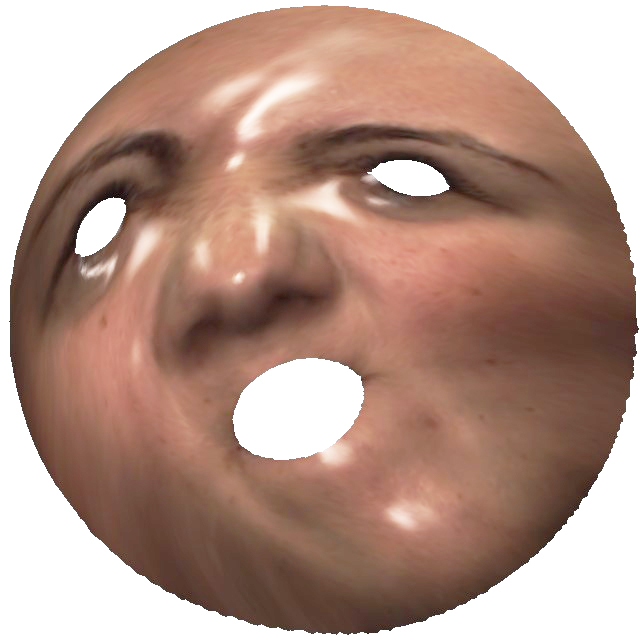
\includegraphics[height=0.25\textwidth]{./figs/roi_face/face_e.jpg}&
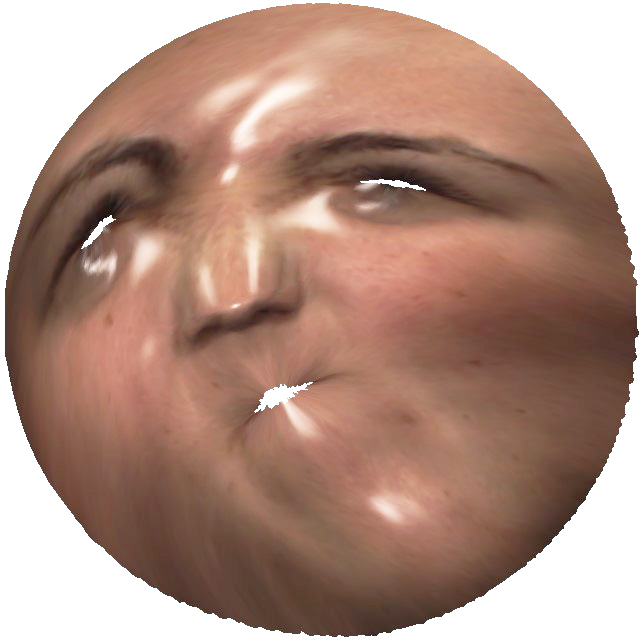
\includegraphics[height=0.25\textwidth]{./figs/roi_face/face_f.jpg}&
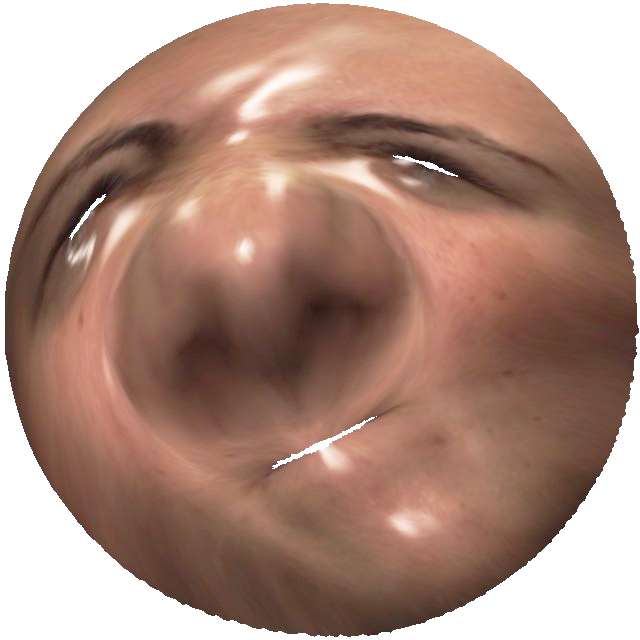
\includegraphics[height=0.25\textwidth]{./figs/roi_face/face_g.jpg}&
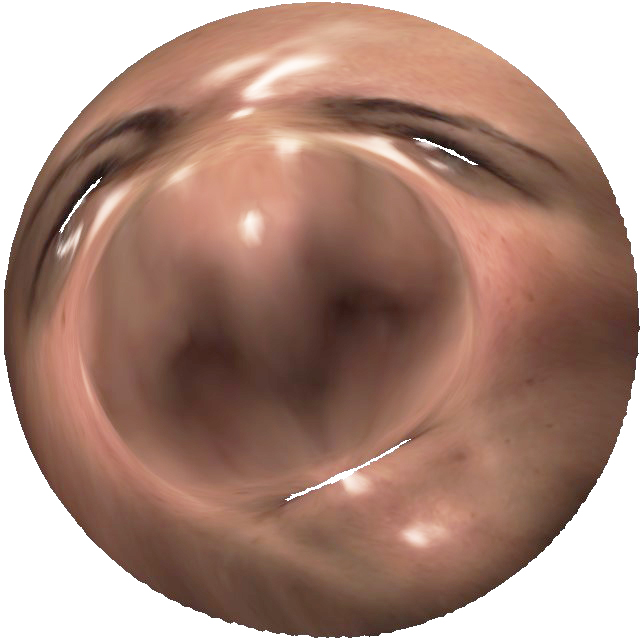
\includegraphics[height=0.25\textwidth]{./figs/roi_face/face_h.jpg}\\
(e)nose:1X,1X &(f) nose:0.25X,0.01X&(g) nose:4X,0.01X&(h) nose:8X,0.01X\\
\end{tabular}
   \caption{Importance driven surface parameterization for human face; (a) the 3d face model; (b)-(d) shows importance driven results of the holes with different scale factors; (e)-(h) shows the importance driven results of the nose and holes with different scale factors.}
  \label{fig:roi_face}
\end{figure}
}


{ \setlength{\tabcolsep}{0pt}
\begin{figure}[!htbp]
\centering
\begin{tabular}{cccc}
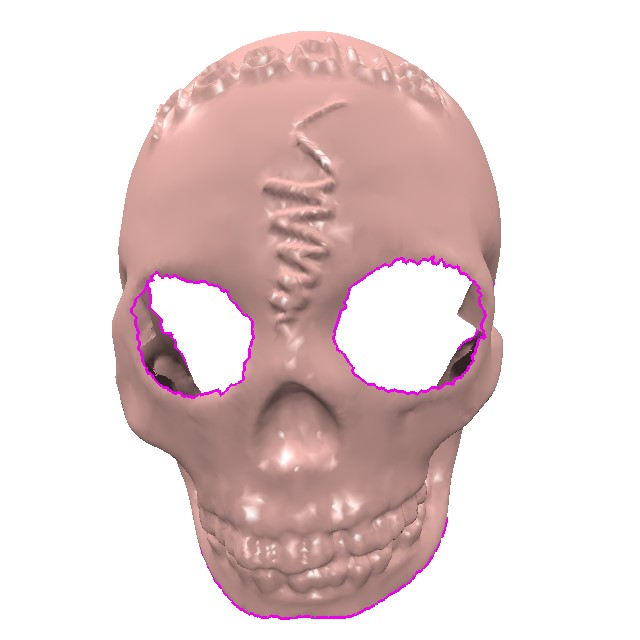
\includegraphics[height=0.25\textwidth]{./figs/roi_skull/skull_a.jpg}&
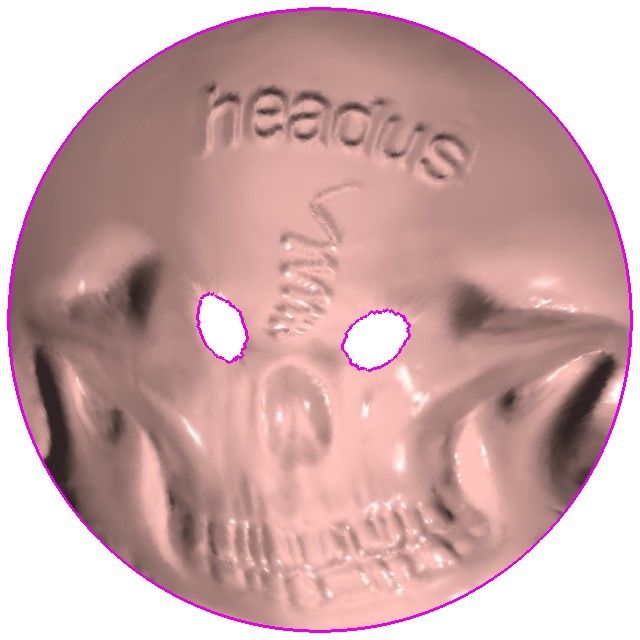
\includegraphics[height=0.25\textwidth]{./figs/roi_skull/skull_b.jpg}&
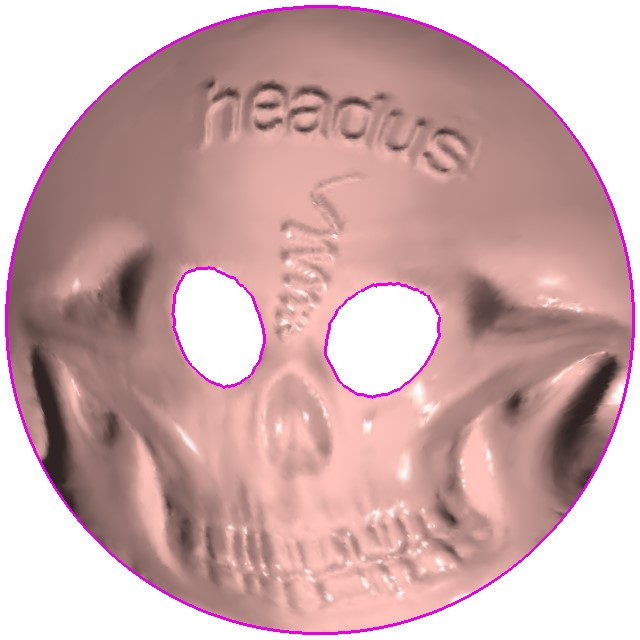
\includegraphics[height=0.25\textwidth]{./figs/roi_skull/skull_c.jpg}&
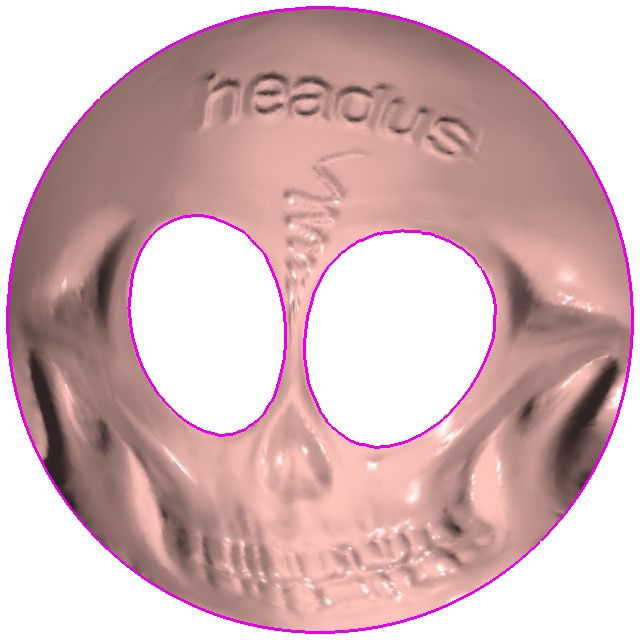
\includegraphics[height=0.25\textwidth]{./figs/roi_skull/skull_d.jpg}\\
(a) 3D skull model &(b)holes:0.25X &(c) holes:1X &(d) holes:4X \\
\end{tabular}
\begin{tabular}{cccc}
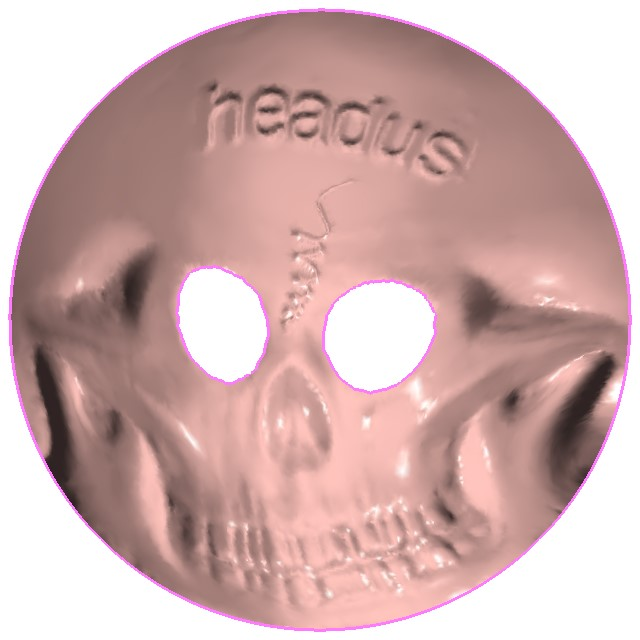
\includegraphics[height=0.25\textwidth]{./figs/roi_skull/skull_e.jpg}&
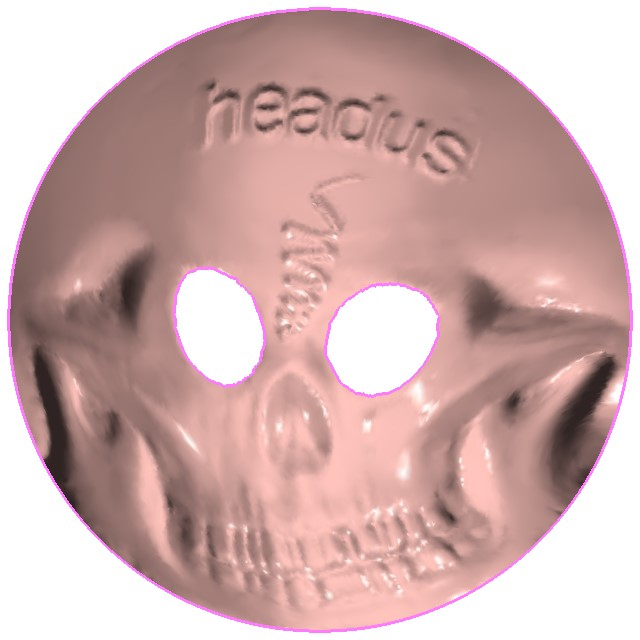
\includegraphics[height=0.25\textwidth]{./figs/roi_skull/skull_f.jpg}&
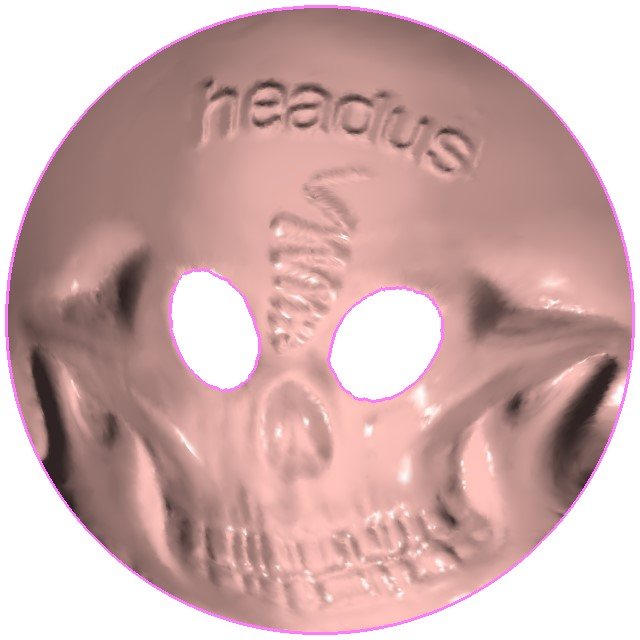
\includegraphics[height=0.25\textwidth]{./figs/roi_skull/skull_g.jpg}&
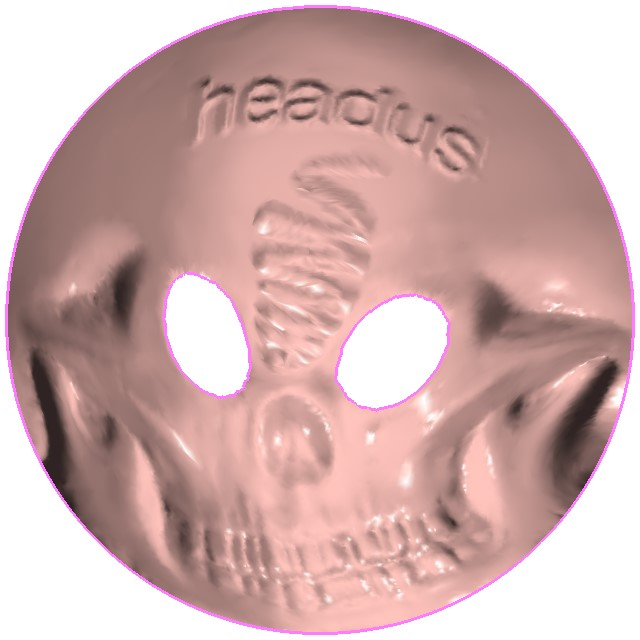
\includegraphics[height=0.25\textwidth]{./figs/roi_skull/skull_h.jpg}\\
(e) curve:0.25X &(f) curve:1X&(g) curve:2X &(h) curve:4X \\
\end{tabular}
   \caption{Importance driven surface parameterization for skull; (a) the 3d skull model; (b)-(d) shows importance driven results of the holes with different scale factors; (e)-(h) shows the importance driven results of the curve with different scale factors.}
  \label{fig:roi_skull}
\end{figure}
}


\subsection{Volume Preserving Parameterization}


In our paper\cite{su2016volume}, our OMT method Fig.[\ref{fig:bunny_omt_morph}] can produce more smooth volume preserving morphing result than Bruno Levy's result Fig.[\ref{fig:bunny_bruno_morph}].



{ \setlength{\tabcolsep}{0pt}
\begin{figure}[!htbp]
\centering
\begin{tabular}{ccccc}
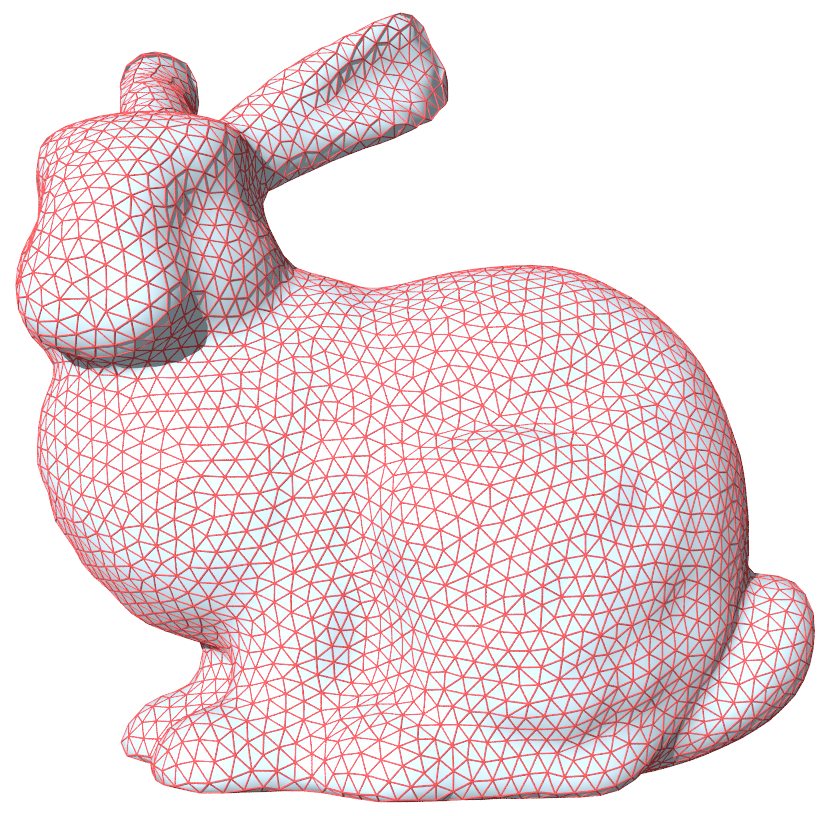
\includegraphics[height=0.2\textwidth]{./figs/bunny_bruno_morph/a.png}&
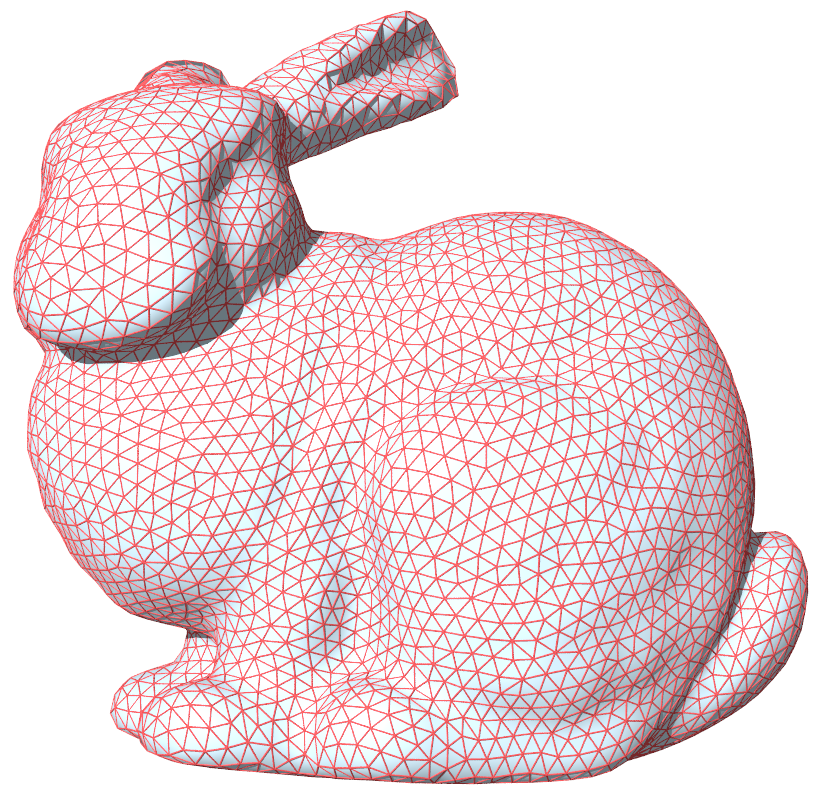
\includegraphics[height=0.2\textwidth]{./figs/bunny_bruno_morph/b.png}&
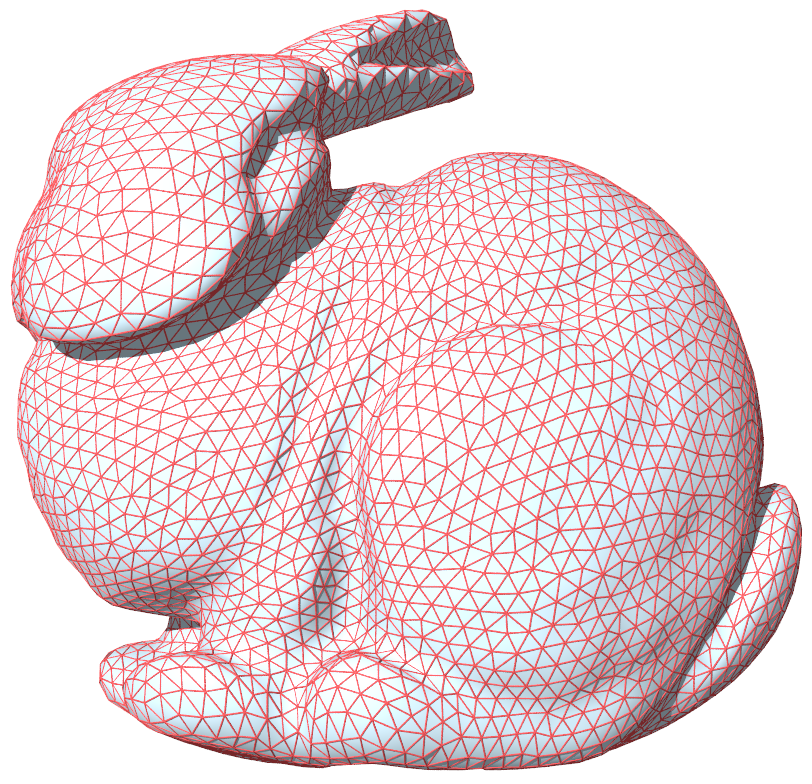
\includegraphics[height=0.2\textwidth]{./figs/bunny_bruno_morph/c.png}&
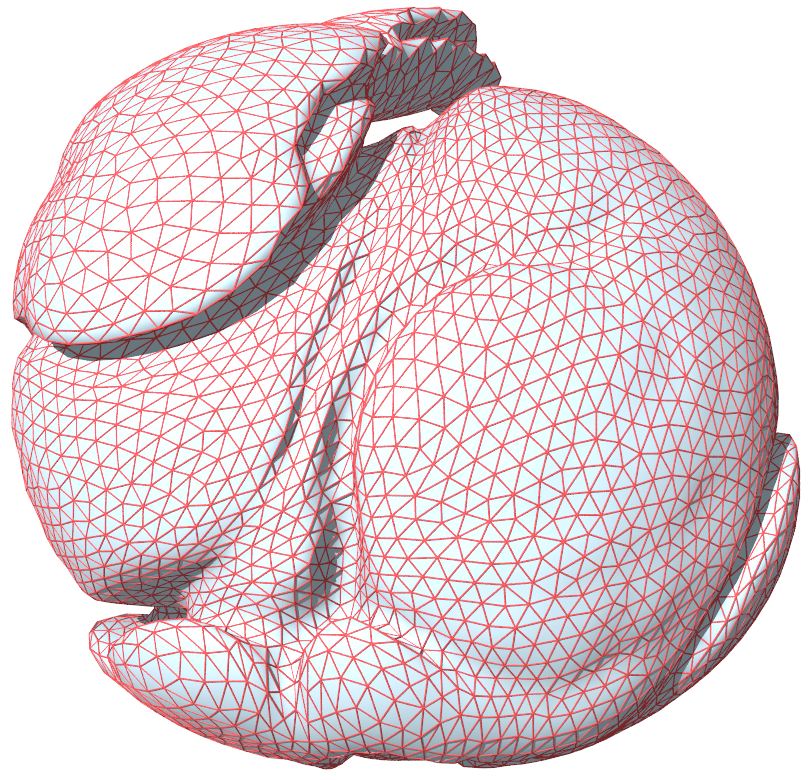
\includegraphics[height=0.2\textwidth]{./figs/bunny_bruno_morph/d.png}&
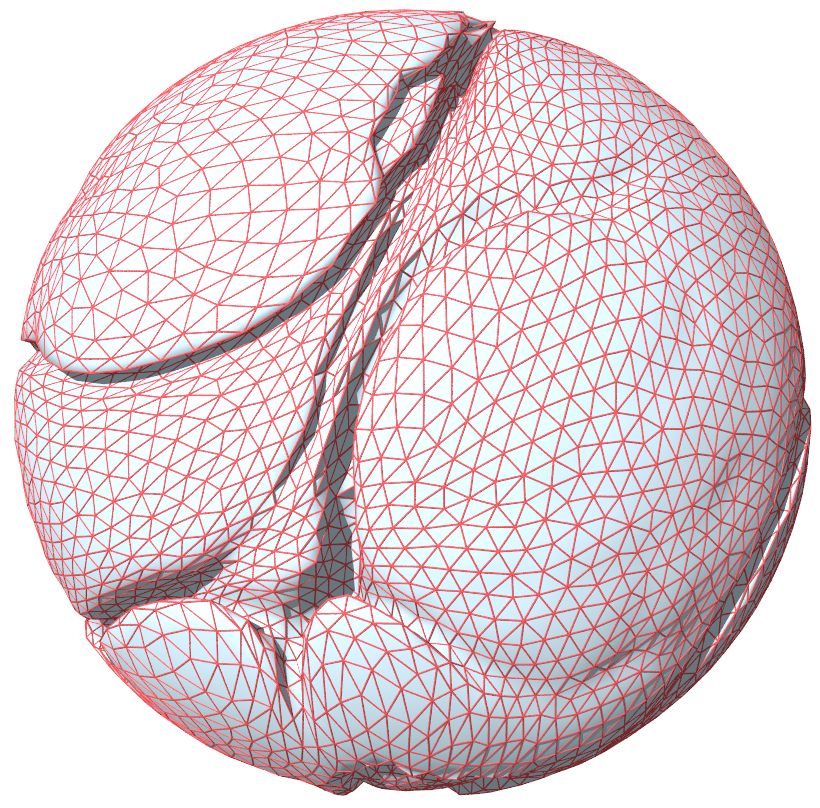
\includegraphics[height=0.2\textwidth]{./figs/bunny_bruno_morph/e.png}\\
\end{tabular}
\begin{tabular}{ccccc}
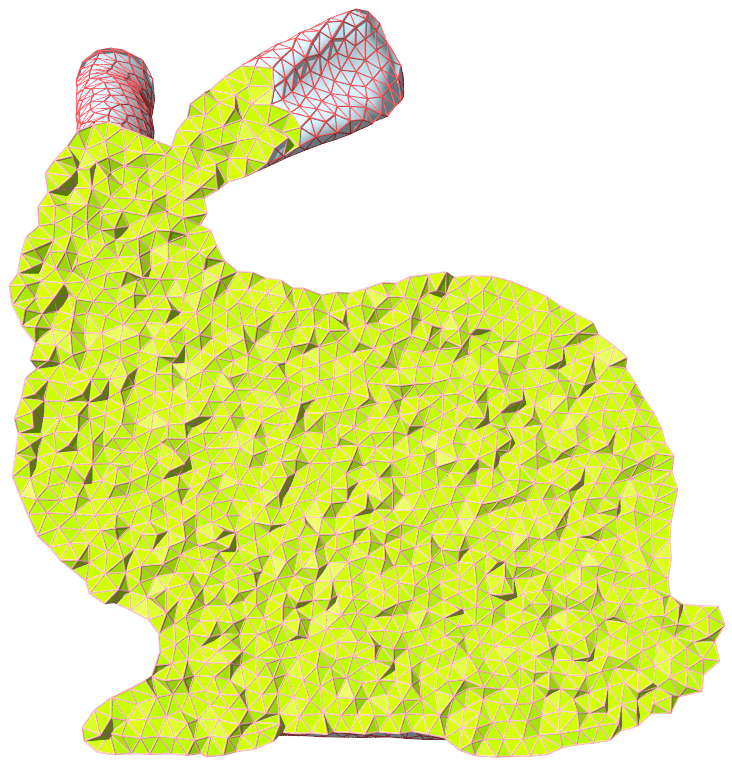
\includegraphics[height=0.2\textwidth]{./figs/bunny_bruno_morph/f.png}&
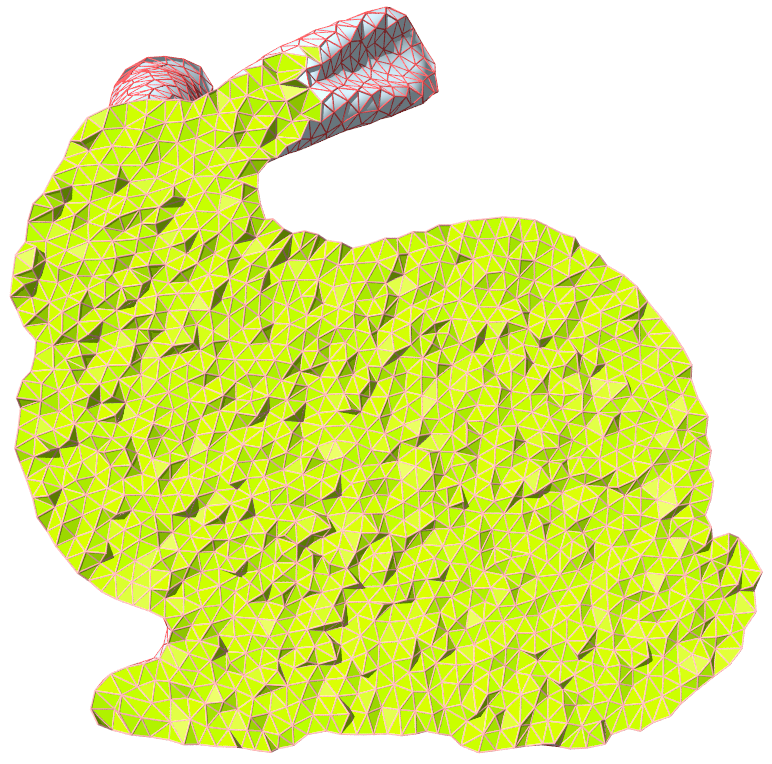
\includegraphics[height=0.2\textwidth]{./figs/bunny_bruno_morph/g.png}&
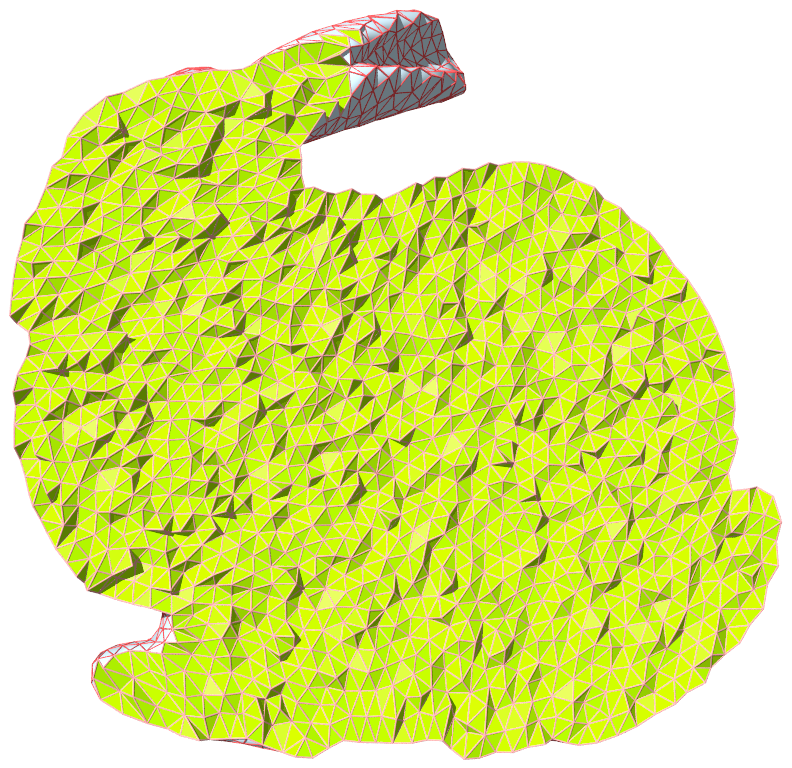
\includegraphics[height=0.2\textwidth]{./figs/bunny_bruno_morph/h.png}&
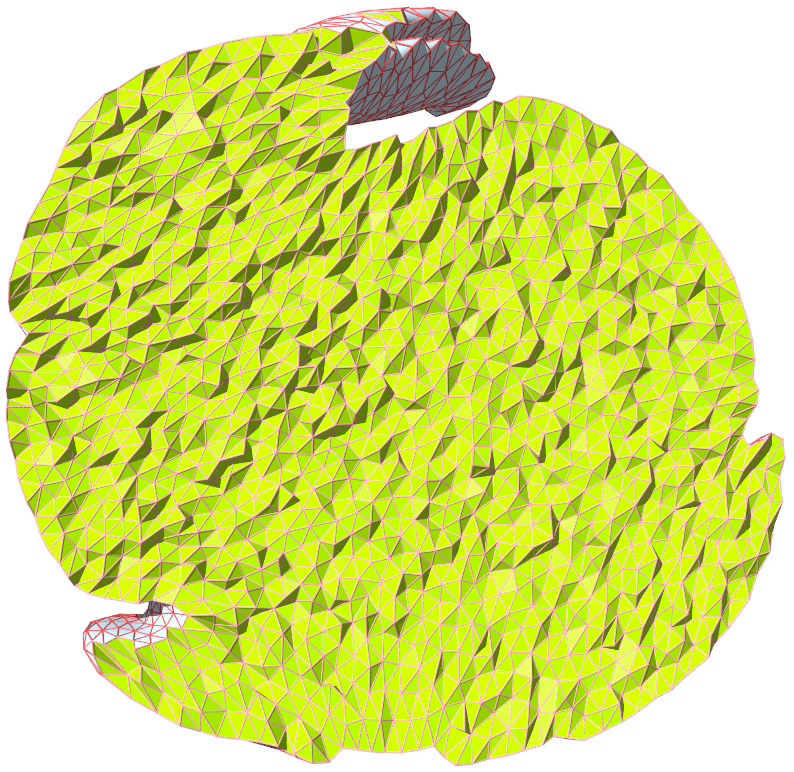
\includegraphics[height=0.2\textwidth]{./figs/bunny_bruno_morph/i.png}&
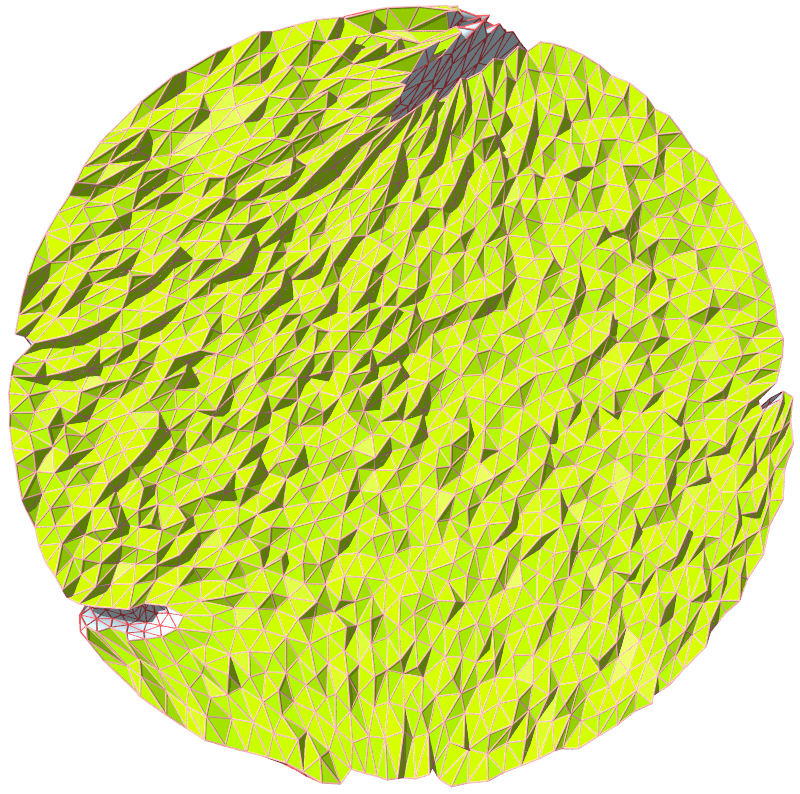
\includegraphics[height=0.2\textwidth]{./figs/bunny_bruno_morph/j.png}\\
(a)t=0 &(b)t=0.25 &(c) t=0.5 &(d) t=0.75 &(e) t=1.0\\
\end{tabular}
  \caption{The volume morphing of Bunny(side view)using Bruno Levy method at typical time}
  \label{fig:bunny_bruno_morph}
\end{figure}
}



{ \setlength{\tabcolsep}{0pt}
\begin{figure}[!htbp]
\centering
\begin{tabular}{ccccc}
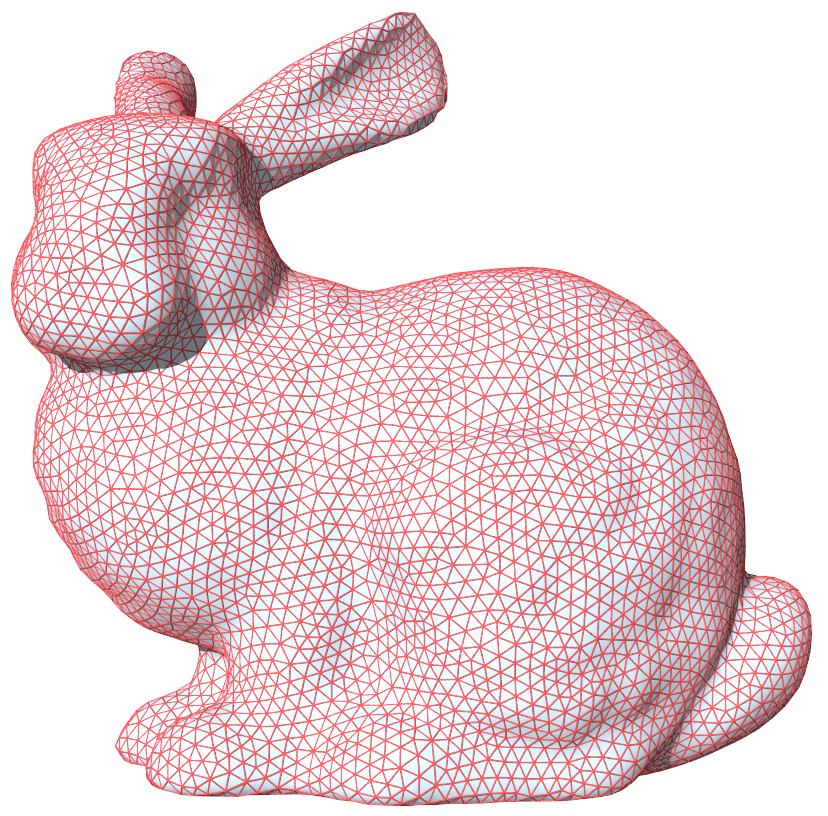
\includegraphics[height=0.2\textwidth]{./figs/bunny_omt_morph/a.png}&
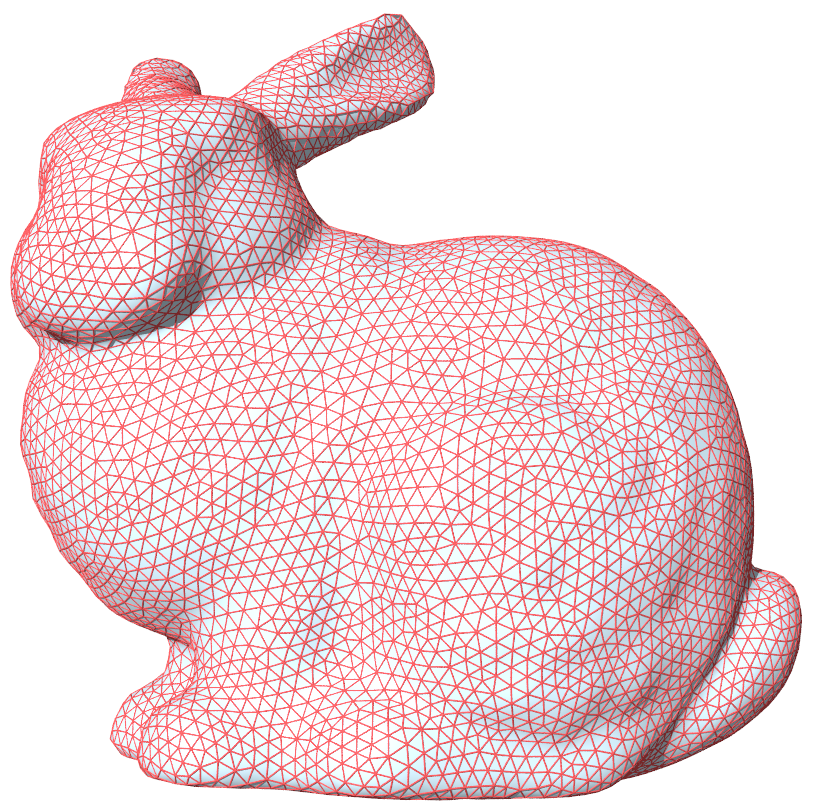
\includegraphics[height=0.2\textwidth]{./figs/bunny_omt_morph/b.png}&
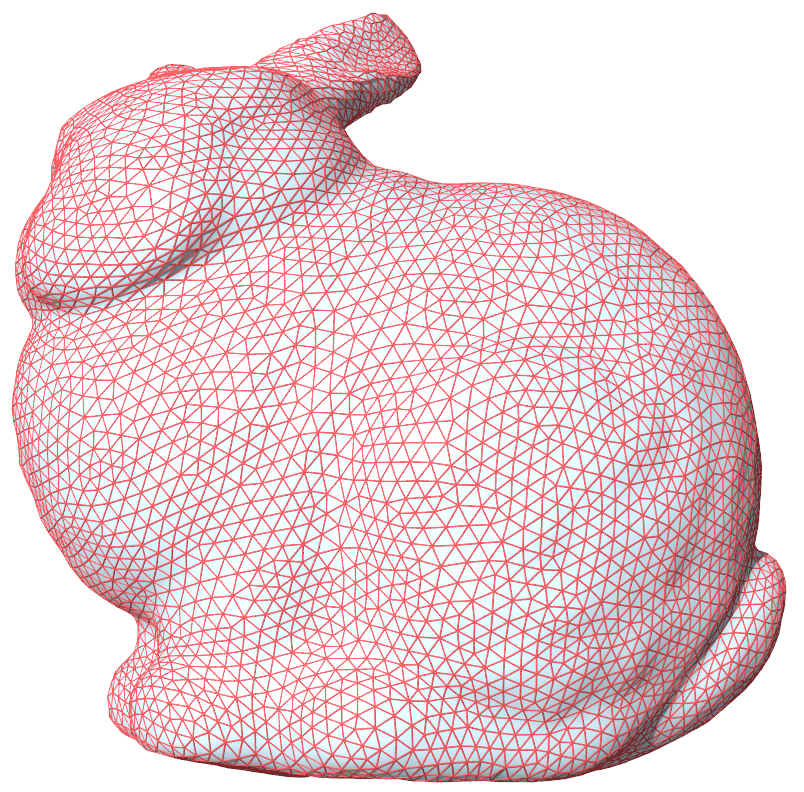
\includegraphics[height=0.2\textwidth]{./figs/bunny_omt_morph/c.png}&
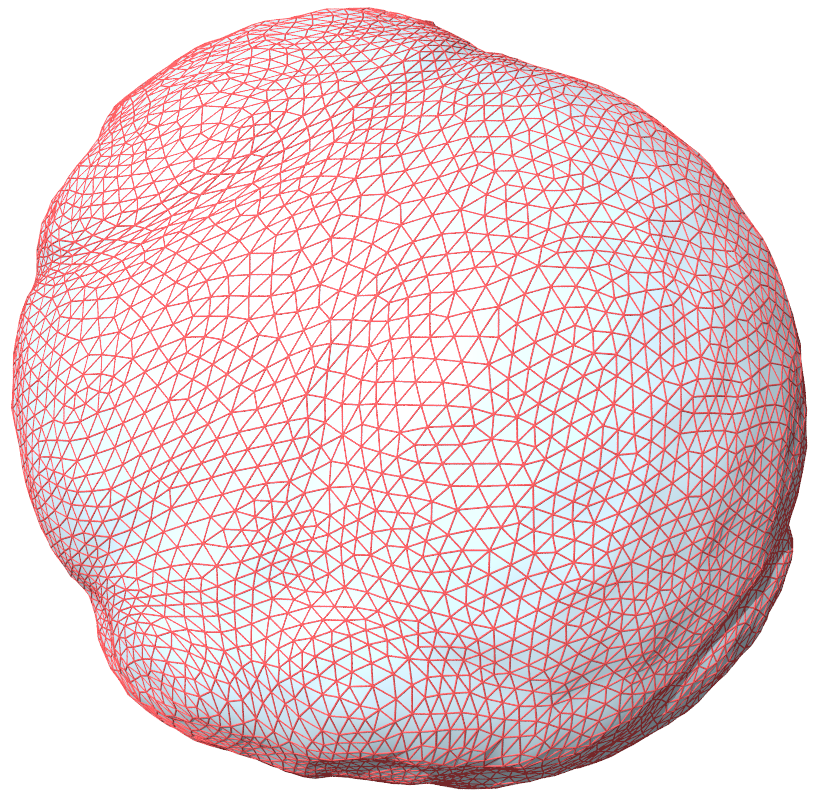
\includegraphics[height=0.2\textwidth]{./figs/bunny_omt_morph/d.png}&
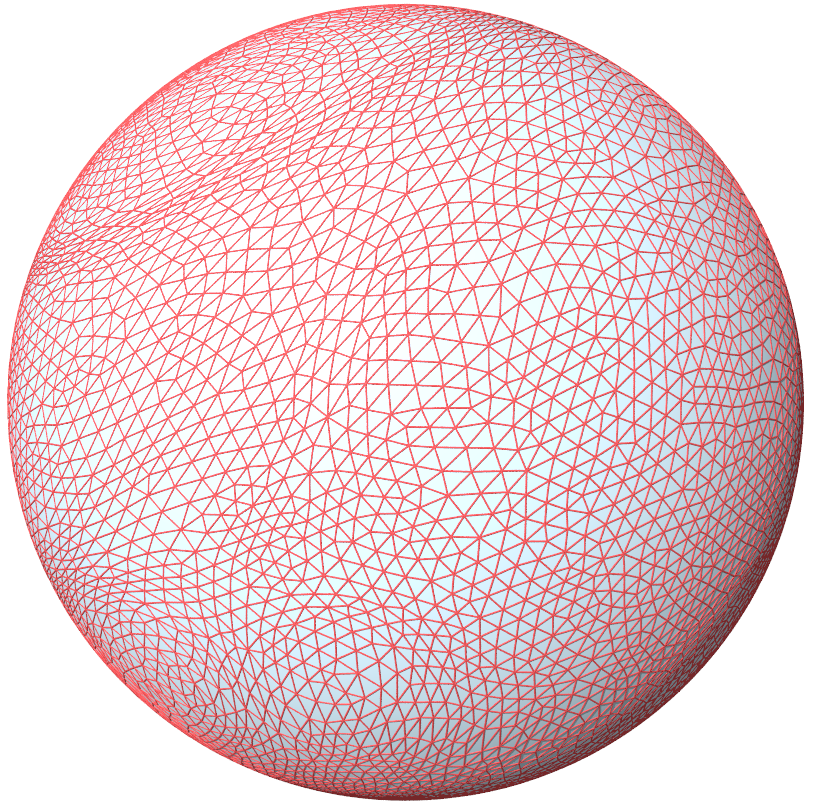
\includegraphics[height=0.2\textwidth]{./figs/bunny_omt_morph/e.png}\\
\end{tabular}
\begin{tabular}{ccccc}
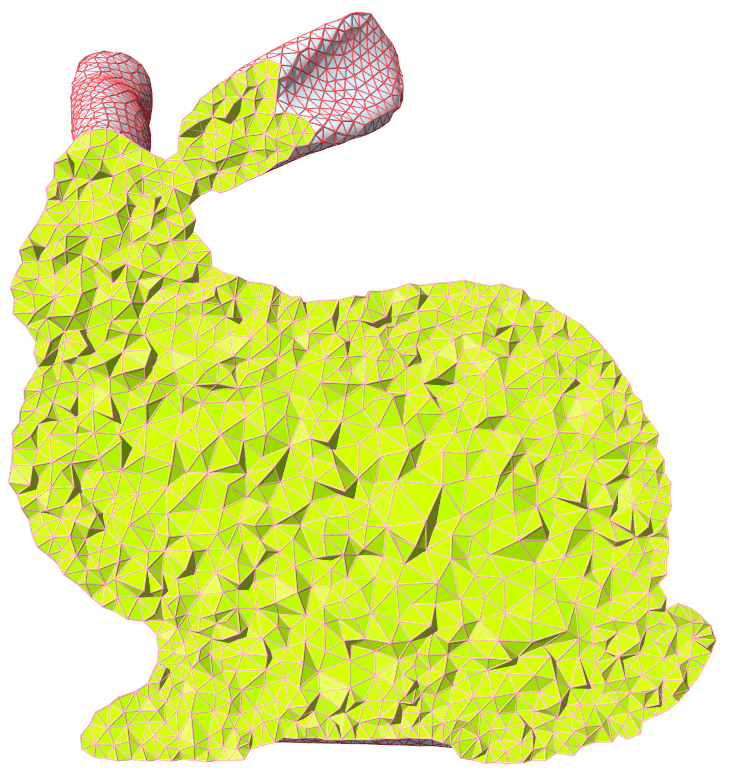
\includegraphics[height=0.2\textwidth]{./figs/bunny_omt_morph/f.png}&
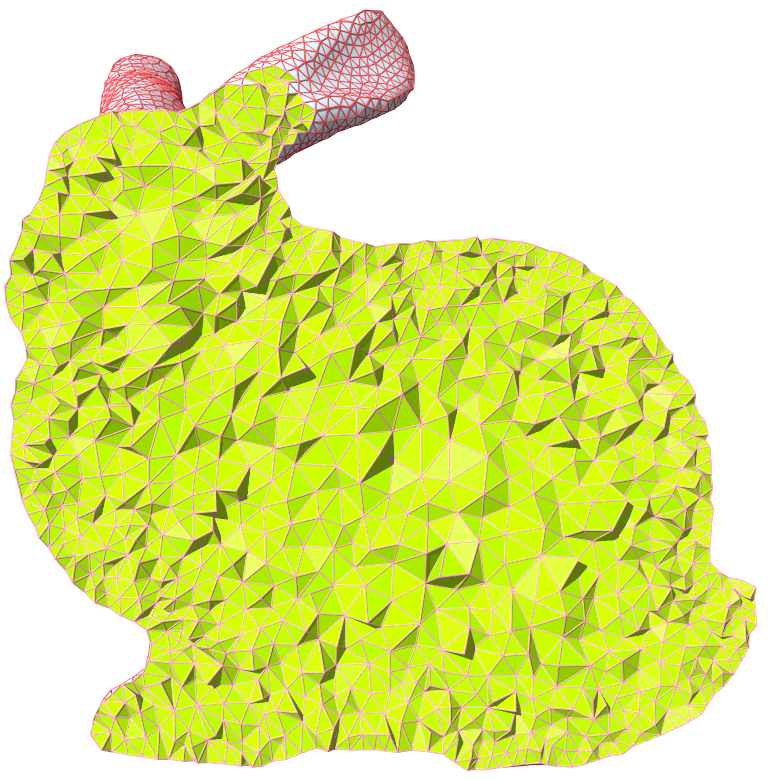
\includegraphics[height=0.2\textwidth]{./figs/bunny_omt_morph/g.png}&
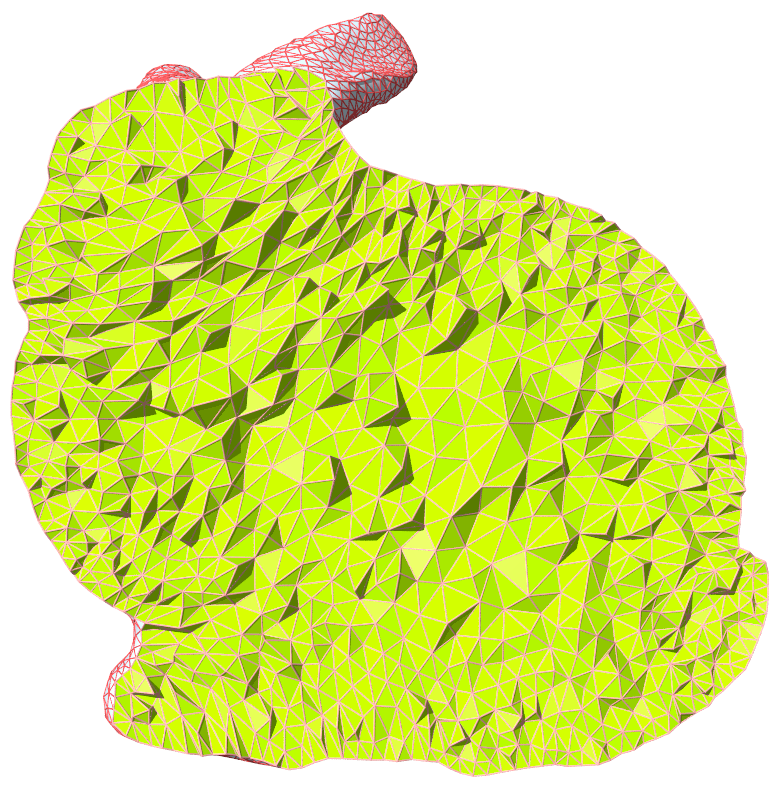
\includegraphics[height=0.2\textwidth]{./figs/bunny_omt_morph/h.png}&
\includegraphics[height=0.2\textwidth]{./figs/bunny_omt_morph/i.png}&
\includegraphics[height=0.2\textwidth]{./figs/bunny_omt_morph/j.png}\\
(a)t=0 &(b)t=0.25 &(c) t=0.5 &(d) t=0.75 &(e) t=1.0\\
\end{tabular}
  \caption{The volume morphing of Bunny(side view)using OMT at typical time }
  \label{fig:bunny_omt_morph}
\end{figure}
}



\section{Conclusion}

In this report, I introduce the history of Optimal Mass Transport(OMT) and our present research approach and experiment result of OMT.

\begin{enumerate}

\item Brenier's polar factorization\cite{brenier1991polar} and Yau-Luo-Gu's\cite{gu2013variational} variational principle method establish the bridge to link  $ Minkowski-Alexandrov $ problem and $ Monge-Kantorovich $ problem.

\item Introduce the Wasserstein distance to describe the similarity of two Riemannian surfaces.

\item OMT and Wasserstein distance's applications in Shape Analysis, Visualization and Volume-Preserving morphing or Volume Parameterization.

\end{enumerate}


\section{Future Work}
In future, there are three directions need more effort.

\begin{enumerate}

\item  High dimension OMT algorithm
\item  OMT Map in $3D$ human face tracking
\item  Volume parametrization
\end{enumerate}


\clearpage
%\bibliographystyle{unsrt}
%\bibliography{egbib}
\bibliographystyle{splncs}
\bibliography{egbib}
\end{document}



